\documentclass{article} % For LaTeX2e
\usepackage{iclr2025_conference,newtxtext,newtxmath}

% % 调整页边距
% \usepackage{geometry}
% \geometry{
%     top=0.85in,      % 稍微减小顶部边距
%     bottom=0.75in,
%     left=0.75in,
%     right=0.75in,
%     includehead,     % 将页眉包含在总高度内
%     headheight=14pt,
%     headsep=0.2in    % 减小页眉和正文的间距
% }
% % 调整行距
% \usepackage{setspace}
% \setstretch{1.0}

% \usepackage{tikz}
% \usetikzlibrary{shapes, arrows.meta, positioning, calc, fit, backgrounds, shadows}

\usepackage{tikz}
\usetikzlibrary{shapes, arrows.meta, positioning, calc, fit, backgrounds, shadows}

% 定义一些绘图样式，保持代码整洁
\tikzset{
    basic/.style={draw, rectangle, rounded corners=2pt, align=center, font=\small},
    input/.style={basic, fill=gray!10, draw=gray!60, inner sep=4pt},
    module/.style={basic, fill=white, draw=black, drop shadow, minimum height=2em},
    tensor/.style={basic, fill=blue!10, draw=blue!40, inner sep=3pt, font=\scriptsize\ttfamily},
    operator/.style={circle, draw, fill=white, inner sep=1pt},
    arrow/.style={->, >=latex, thick, color=black!70}
}
% Optional math commands from https://github.com/goodfeli/dlbook_notation.
\input{math_commands.tex}

\usepackage{hyperref}
\usepackage{url}
\usepackage{booktabs}
\usepackage{graphicx}


\title{A Case Study on Generalization Challenges in Imitation Learning: \\ Architecture Choices, Distribution Design, and Data Scaling for Robust Robotic Manipulation}

% Authors must not appear in the submitted version. They should be hidden
% as long as the \iclrfinalcopy macro remains commented out below.
% Non-anonymous submissions will be rejected without review.

% \author{Qiming Qiu(23307110278), Zhipeng Xu(23307110122)
% }
\author{Qiming Qiu \\ \texttt{23307110278@m.fudan.edu.cn} \And Zhipeng Xu \\ \texttt{23307110122@m.fudan.edu.cn}
}

% The \author macro works with any number of authors. There are two commands
% used to separate the names and addresses of multiple authors: \And and \AND.
%
% Using \And between authors leaves it to \LaTeX{} to determine where to break
% the lines. Using \AND forces a linebreak at that point. So, if \LaTeX{}
% puts 3 of 4 authors names on the first line, and the last on the second
% line, try using \AND instead of \And before the third author name.

\newcommand{\fix}{\marginpar{FIX}}
\newcommand{\new}{\marginpar{NEW}}
\usepackage{subcaption}
\iclrfinalcopy % Uncomment for camera-ready version, but NOT for submission.
\begin{document}


\maketitle

\begin{abstract}
Imitation learning from human demonstrations is an effective approach for teaching robotic manipulation skills. However, due to the absence of explicit reward functions that convey how a task should be performed, imitation learning often exhibits poorer robustness than reinforcement learning when faced with out-of-distribution scenarios, limiting its applicability in real-world environments. This challenge is further exacerbated when learning visual policies, where the high-dimensional inputs significantly increase training difficulty and visual variations such as lighting and texture, together with physical discrepancies between simulation and reality, give rise to the well-known sim-to-real gap. Addressing these issues typically requires large-scale and diverse expert datasets, yet data collection is particularly challenging for complex systems involving dual-arm manipulation and multi-fingered hands. Automated data generation in simulation therefore provides a scalable and compelling alternative. In this work, we first empirically analyze the difficulty of generalizing imitation learning policies on a Franka Panda robot in PyBullet, and demonstrate that a combination of generalization techniques can substantially improve policy robustness. These findings motivate the use of expert data augmentation, expanded object pose distributions, and enhanced visual generalization. Building on these insights, we leverage MimicGen for data augmentation and Cosmos Transfer for visual generalization, and ultimately obtain robust manipulation policies in Isaac Sim.

\end{abstract}

\section{Introduction}
Learning with real robots requires careful consideration of potentially dangerous or unexpected behaviors, especially in safety-critical applications\cite{JMLR:v16:garcia15a}. As a result, learning algorithms are often applied in simulation environments such as PyBullet, Gazebo, and Isaac Sim. While simulation-based training enables large-scale data collection at low cost, the transfer of learned policies to the real world remains challenging due to inherent mismatches between simulated and real environments. Bridging this simulation-to-reality gap requires methods that can account for discrepancies in both sensing and actuation. Actuation mismatches can be partially mitigated by increasing the physical realism of simulators\cite{zhao2020closingsimtorealgapcollaborative}. Existing approaches commonly introduce environmental perturbations or rely on domain randomization techniques\cite{Muratore_2021}\cite{ramakrishnan2020blind}. Beyond these factors, agents deployed in real-world settings inevitably encounter novel situations that were not present during training  {Ramya2026}, and may need to adapt their policies to a broader set of tasks. 

While simulation fidelity constrains policy generalization, the choice of learning paradigm plays a critical role in robustness under out-of-distribution conditions. Compared to reinforcement learning—which often demands extensive reward engineering and long training cycles to mitigate reward sparsity and overfitting—imitation learning from human demonstrations offers a more direct and efficient approach to acquiring manipulation skills\cite{torne2024reconcilingrealitysimulationrealtosimtoreal}\cite{wang2025recipeefficientsimtorealtransfer}. However, as a supervised regression framework, imitation learning lacks explicit reward signals that encode why certain behaviors are preferable, and instead purely mimics expert demonstrations. Consequently, policies learned via imitation learning tend to degrade sharply when encountering scenarios beyond the training distribution, unless trained on large-scale demonstration datasets.

Thus, the question “How difficult is it to train a robotic arm to perform a simple task via imitation learning in a controlled simulation?” can be answered as follows: {\bf it may seem easy to train, but improving generalization remains a fundamental challenge}. Addressing this issue requires expert datasets that are both large in scale and diverse in distribution, yet data collection remains a major bottleneck. To reduce reliance on real-world data, recent works have explored automated data augmentation and synthetic data generation. For instance, MimicGen expands a small set of real teleoperation trajectories into thousands of demonstrations via interpolation, while world-model-based approaches such as Cosmos generate simulation data from multimodal inputs (e.g., segmentation, depth, and edges), alleviating the synthetic-to-real gap inherent in conventional CG-based simulators\cite{zhang2025stepworldmodelssurvey}.

Motivated by these observations, this work systematically studies the generalization capability of imitation learning for robotic manipulation. We conduct controlled evaluations on robotic arms, introduce multiple complementary generalization techniques, and empirically validate their effectiveness.

\textbf{ The main contributions of this paper are as follows:}

\begin{minipage}{\linewidth}
\begin{itemize}
\item  We develop a manipulation training framework for the Franka Panda robot in PyBullet and propose a set of techniques to improve policy generalization. These include high-resolution visual representations, spatial feature extraction via Spatial Softmax, and dense phase supervision to alleviate perceptual ambiguity. Experimental results show that the resulting visual policy achieves a robust success rate of 84.8\% under fully randomized environments, and demonstrates strong adaptability to variations in lighting, physical friction, and sensor noise in gradient-based generalization tests.Furthermore, we conduct a thorough evaluation of the impact of training algorithm selection and training data distribution diversity on model performance, providing valuable guidance for the development and scaling of more complex manipulation policies in future work.

\item  We build a complete data diversity enhancement pipeline in Isaac Sim by integrating MimicGen\cite{jiang2025dexmimicgenautomateddatageneration} for trajectory interpolation-based augmentation and Cosmos Transfer\cite{nvidia2025cosmosworldfoundationmodel} for visual domain randomization. Starting from only 10 real teleoperation trajectories, MimicGen expands the dataset to 2,000 trajectories, enabling a trained policy to achieve a 97.0\% success rate and validating the effectiveness of the augmented data. Further visual generalization through Cosmos Transfer enhances the policy’s potential for real-world deployment.
\end{itemize}
\end{minipage}
\section{Related Work}

{\bfseries Data Collection through Teleoperation.}Teleoperation is a widely adopted approach for collecting task demonstrations in robotics\cite{zhang2018deepimitationlearningcomplex} . In this paradigm, human operators remotely control a robot in real time via an interface, while sensor observations and control commands are recorded to construct a dataset.

{\bfseries Imitation Learning.}Behavioral Cloning (BC) is a canonical framework for learning robot control policies from demonstrations and has been extensively explored in prior work\cite{Pomerleau2015ALVINNAA} .  Despite its simplicity and effectiveness, BC often suffers from limited robustness under distribution shift, motivating research into data diversity and generalization-enhancing techniques.

{\bfseries Data Augmentation.}Recent studies have leveraged affine and appearance-based data augmentation techniques to increase dataset size and diversity \cite{dalal2023imitatingtaskmotionplanning} \cite{wang2025recipeefficientsimtorealtransfer}. DexMimicGen generates augmented datasets through online simulation, ensuring that synthesized trajectories remain physically valid \cite{jiang2025dexmimicgenautomateddatageneration}.

{\bfseries World Generation Model.}World models have recently emerged as a promising paradigm for data-driven simulation.Cosmos-Transfer\cite{nvidia2025cosmosworldfoundationmodel}, a key branch of Cosmos World Foundation Models, specializes in multimodal, controllable conditional world generation and world-to-world transfer through the use of ControlNet-based architectures.

%% Please note that we have introduced automatic line number generation
%% into the style file for \LaTeXe. This is to help reviewers
%% refer to specific lines of the paper when they make their comments. Please do
%% NOT refer to these line numbers in your paper as they will be removed from the
%% style file for the final version of accepted papers.

% Authors are required to use the ICLR \LaTeX{} style files obtainable at the
% ICLR website. Please make sure you use the current files and
% not previous versions. Tweaking the style files may be grounds for rejection.

\section{Environment \& Method}
\begin{figure}[ht]
\centering
\begin{subfigure}[t]{0.48\textwidth}
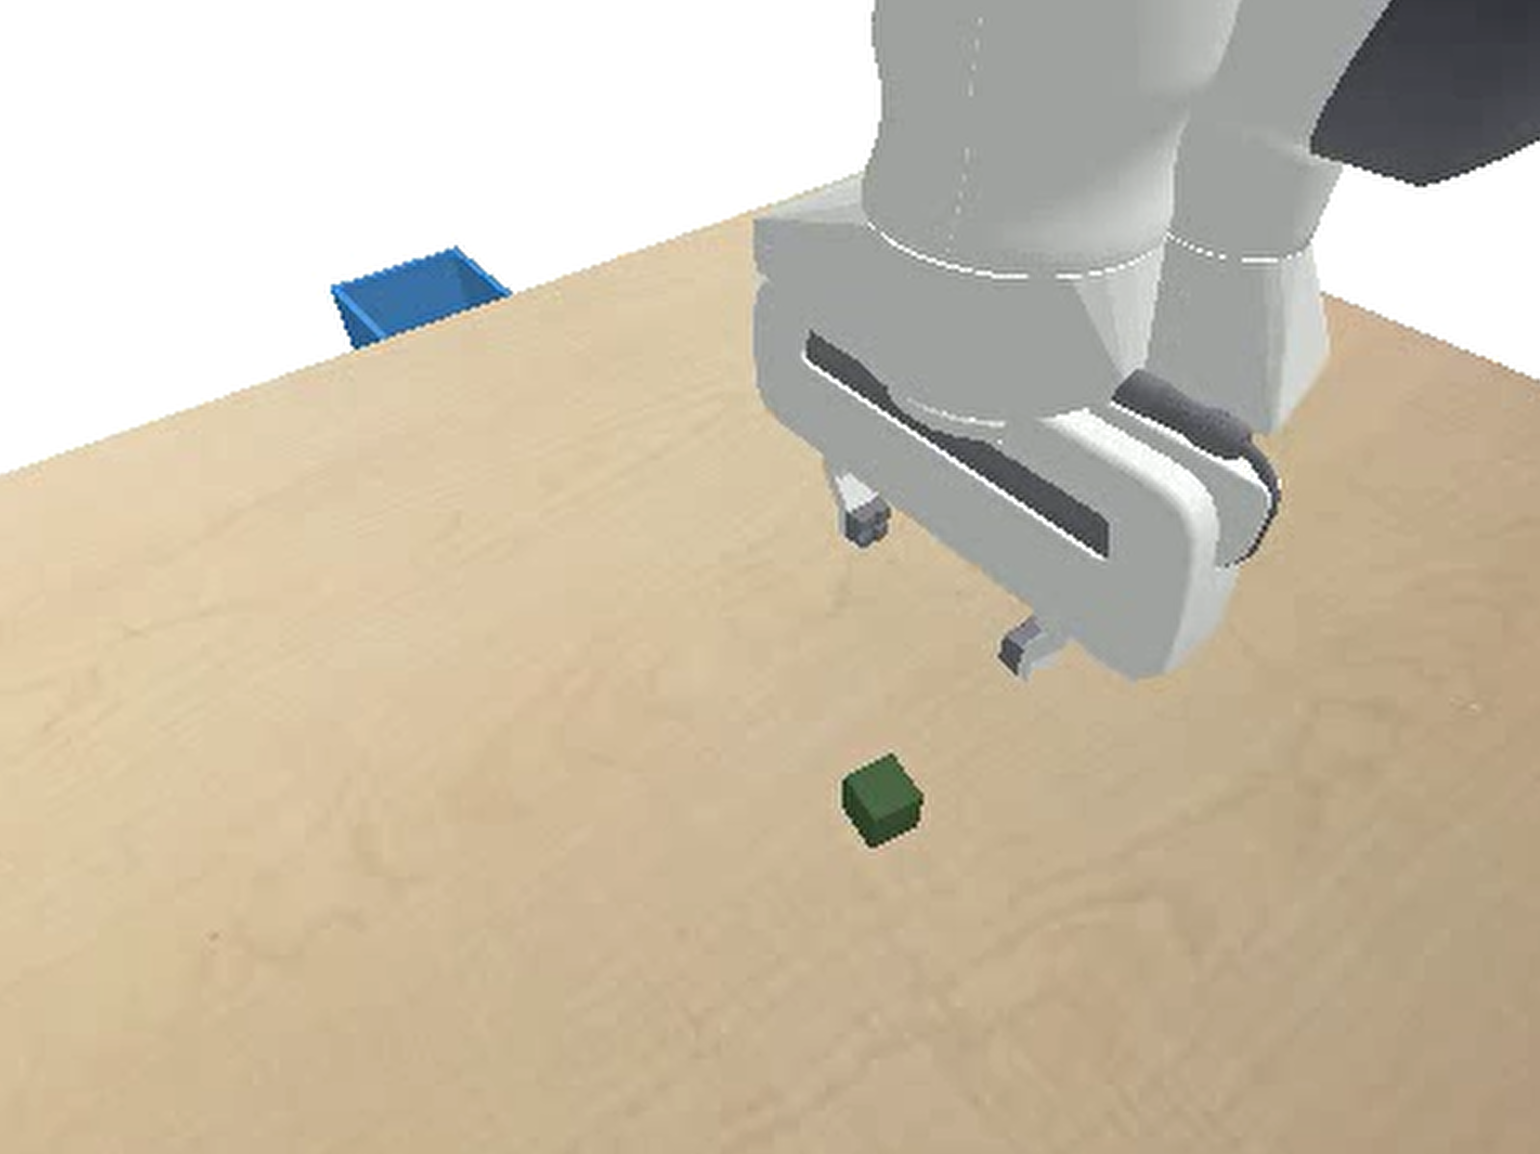
\includegraphics[width=0.8\linewidth]{pic/Enironment setting.png} 
\caption{The simulated desktop manipulation environment in PyBullet. A 7-DoF Franka Panda robot arm is tasked to pick up a randomized cube on the table and place it into the blue basket.}
\label{fig:env_setup}
\end{subfigure}
\hfill  % 強制一點水平間距
    \begin{subfigure}[t]{0.48\textwidth}
        \centering
        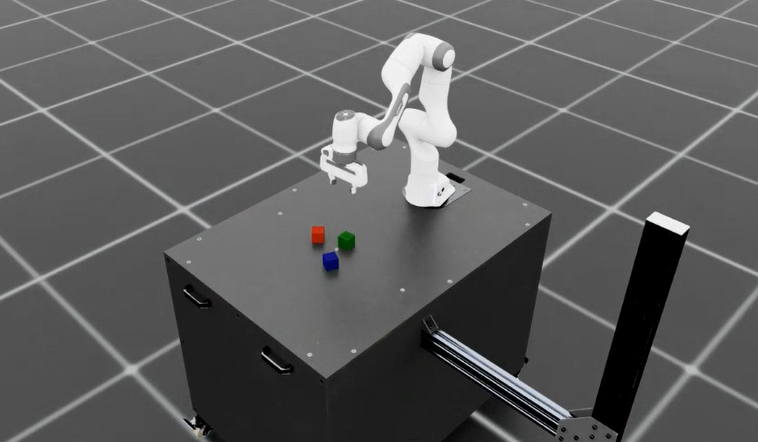
\includegraphics[width=\linewidth]{pic/Isaac setting.png} 
        \caption{The simulated desktop manipulation environment in Isaac Sim.Franka Panda robot arm is tasked to pick up randomized cubes and stack them in order.}
        \label{fig:Isaac setting}
    \end{subfigure}
\end{figure}

\subsection{Task setting}
We constructed a desktop manipulation scenario in the PyBullet physics engine, featuring a 7-DoF Franka Emika Panda robotic arm equipped with a parallel-jaw gripper. The primary task is a challenging Pick-and-Place operation: the arm must grasp a cube (Cube) located at a randomized initial position on the table and precisely place it into a container (Basket) whose position is also randomized.

To further demonstrate the effectiveness of our proposed generalization measures under more demanding conditions, we designed a longer-horizon and more complex task in Isaac Sim: stacking three cubes (Stack) in a vertical sequence from bottom to top, requiring precise alignment, stable grasping, and sequential placement while maintaining stability throughout the multi-step process.
\subsection{Data collection}
We employed a dual strategy for data acquisition, combining scripted expert demonstration generation with human teleoperation, as detailed below.

{\bf Expert Demonstration Generation.}For the Pick-and-Place task in PyBullet, we implemented a multi-phase scripted expert policy inspired by human claw-machine operation, divided into seven distinct phases: (1) rapid approach to the cube overhead, (2) slow descent toward the cube, (3) grasp closure, (4) lift, (5) rapid transport to the target overhead, (6) slow descent to the basket, and (7) release. In the Vision-Final variant, we additionally incorporated two slow alignment phases: one for precise centering above the cube and another for fine alignment above the basket.To narrow the sim-to-real gap and promote realistic, human-like behavior, we deliberately avoided perfect, noise-free trajectories. Instead, we designed a data generation pipeline incorporating anthropomorphic perturbations. Using a RandomizationConfig, we collected 1000 demonstration trajectories while injecting the following key noise sources (summarized in Table 1):
At every timestep: Gaussian noise (std = 0.002, probability = 0.3) and Ornstein–Uhlenbeck (OU) noise (regression coefficient = 0.15, diffusion coefficient = 0.003)

Initial conditions: randomized gripper starting pose, cube position and size, basket position, followed by inverse kinematics (IK) reachability validation to ensure feasibility.

To enrich the training distribution and prevent the policy from memorizing fixed relative offsets, we applied extensive randomization to object initial poses. In addition to the baseline cube position range ($  x \in [0.25, 0.65]  $) and size scaling, we introduced basket\_pos\_x\_noise = 0.08 ($  \pm  $ 8 cm). This forces the model to rely on visual localization of the basket rather than hardcoded movements, significantly enhancing spatial generalization.
\begin{figure}[ht]
\centering

\begin{minipage}[t]{0.18\textwidth}
    \centering
    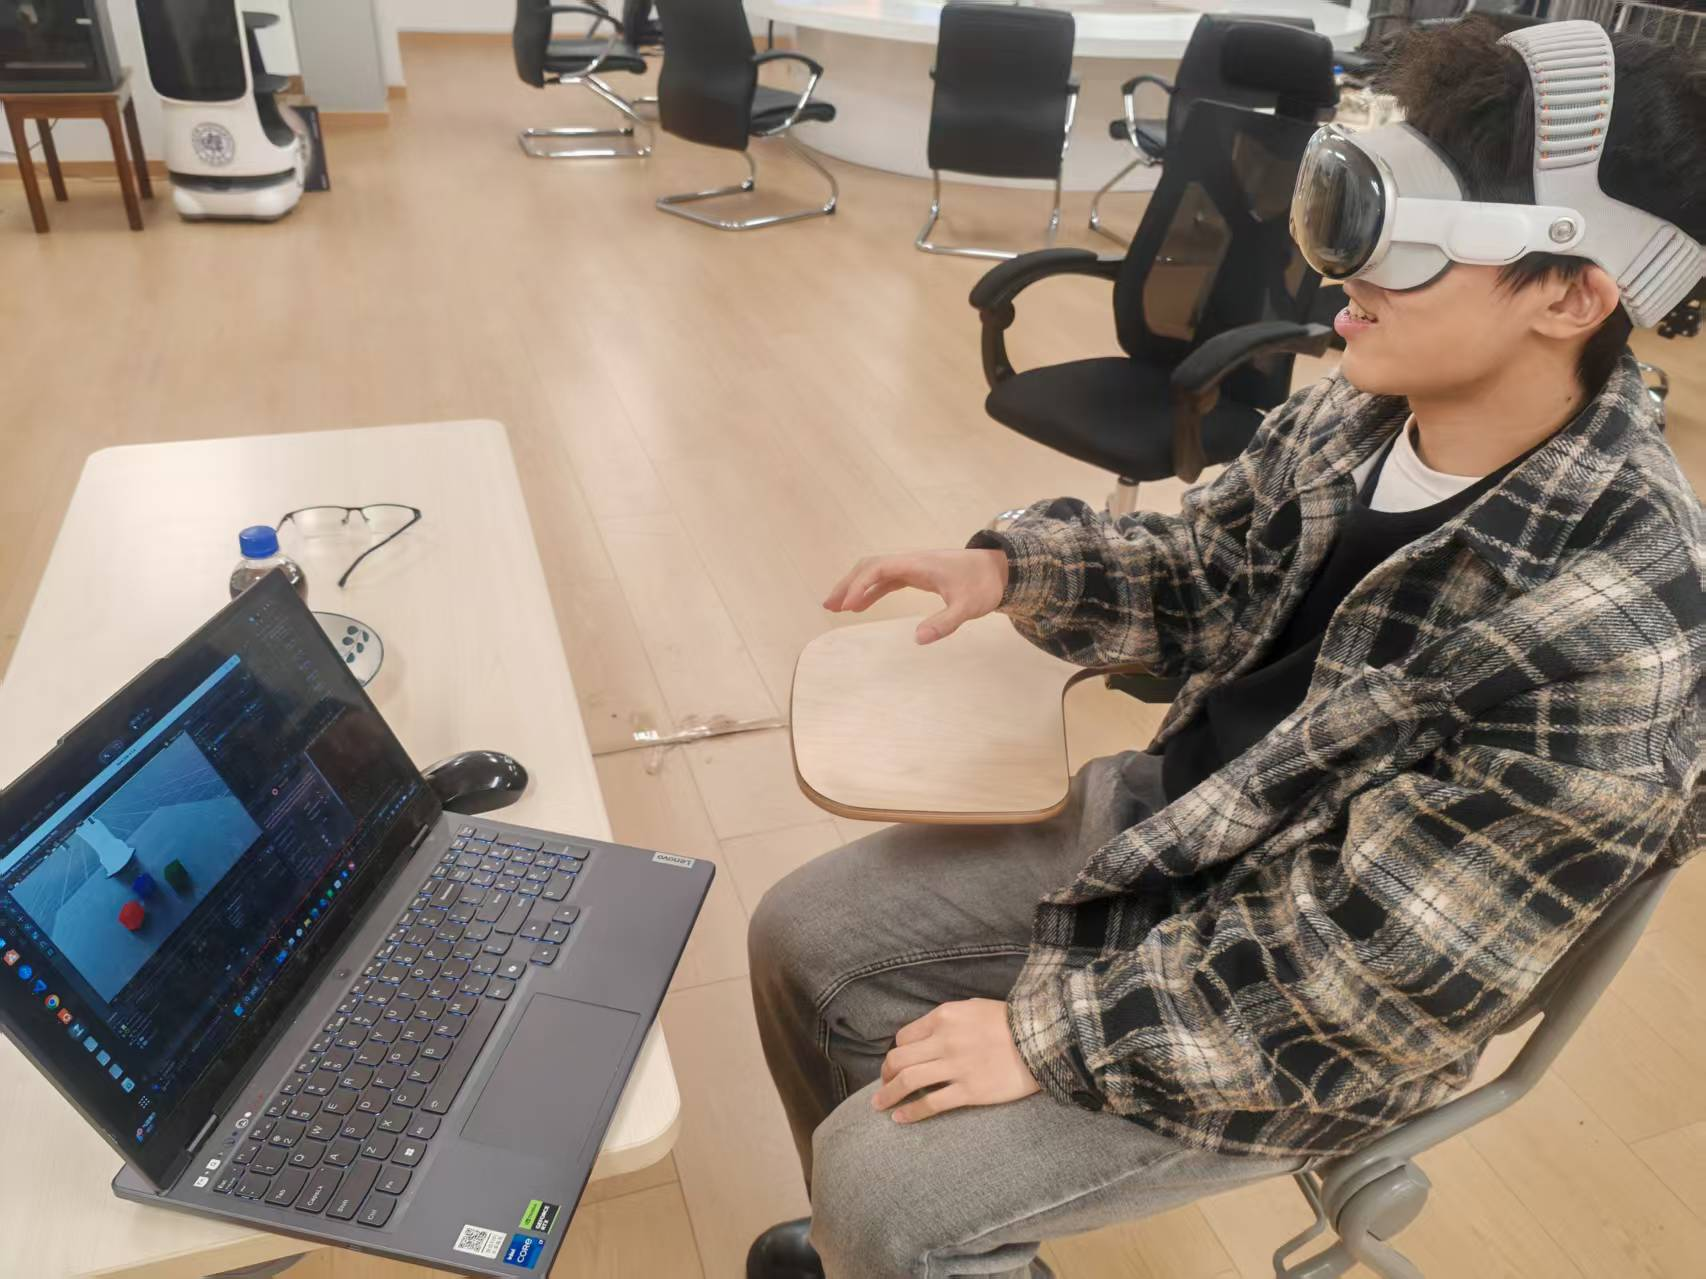
\includegraphics[width=\linewidth]{pic/teleop.jpg}
    \vspace{0.5ex}  % 微調 caption 上方空間
    \caption{\footnotesize Data collection via Apple Vision Pro teleoperation.}
    \label{fig:teleop_interface}
\end{minipage}%
\hspace{1em}%  ← 只用小間距，不要用 \hfill
\begin{minipage}[t]{0.78\textwidth}
    \centering
    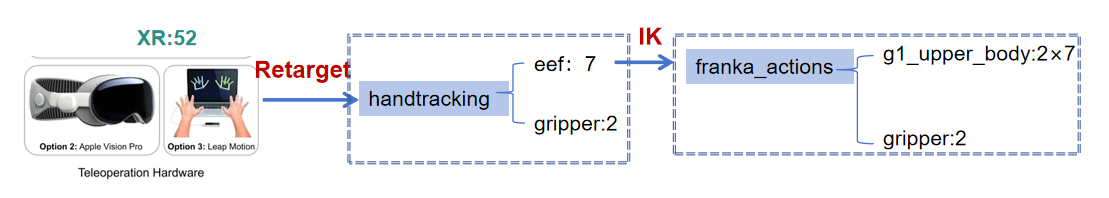
\includegraphics[width=\linewidth]{pic/teleop pipeline.png}
    \vspace{0.5ex}
    \caption{\footnotesize Complete pipeline: Vision Pro hand tracking → OpenXR → coordinate transformation \& kinematic retargeting → smooth joint commands for Franka Panda arm.}
    \label{fig:teleop_pipeline}
\end{minipage}
\end{figure}

{\bf Human Teleoperation Data Collection.}For the more complex stacking task in Isaac Sim, where scripted multi-phase generation is impractical, we utilized Apple Vision Pro for high-fidelity human demonstration collection. Hand pose data (26-DoF joint positions per hand) were captured via OpenXR tracking, retargeted to the parallel-jaw gripper's 2-DoF action and the 7-DoF end-effector pose, and then solved via inverse kinematics to obtain the corresponding 7-DoF joint actions for the Franka Panda.Building on the substantial performance gains observed from distribution augmentation in PyBullet experiments, we randomized the initial positions of the three cubes within a 0.2 × 0.2 m area on the table. This randomization introduces meaningful variability in relative placements, grasp sequences, and stacking order, while remaining within kinematically feasible bounds. All collected teleoperated trajectories were successful, high-quality demonstrations suitable for direct imitation learning.


\subsection{Policy Learning}
\label{sec:policy_learning}

\subsubsection{Observation Space Definition}
To systematically evaluate the impact of perceptual modalities, we define two distinct observation spaces.

{\bfseries 1. Privileged State Space ($\mathcal{O}_{priv}$):} 
This low-dimensional space provides ground-truth physical states, serving as a "teacher" configuration. It is defined as:
\begin{equation}
    \mathbf{s}_{priv} = [\mathbf{q}, \dot{\mathbf{q}}, \mathbf{x}_{ee}, \mathbf{x}_{obj}^{ee}, \mathbf{x}_{target}^{ee}] \in \mathbb{R}^{d_{priv}}
\end{equation}
where $\mathbf{q}, \dot{\mathbf{q}}$ are joint positions and velocities, $\mathbf{x}_{ee}$ is the end-effector pose, and critically, $\mathbf{x}_{obj}^{ee}$ and $\mathbf{x}_{target}^{ee}$ denote the relative positions of the object and target with respect to the end-effector. This space is fully observable and Markovian.

{\bfseries 2. Visual Observation Space ($\mathcal{O}_{vis}$):} 
This space represents the realistic sensor interface for deployment. It relies solely on ego-centric sensors:
\begin{equation}
    \mathbf{o}_{vis} = [\mathbf{I}_{front}, \mathbf{I}_{wrist}, \mathbf{p}_{proprio}]
\end{equation}
where $\mathbf{I} \in \mathbb{R}^{4 \times 112 \times 112}$ represents the stacked RGB-D images from two camera views, and $\mathbf{p}_{proprio}$ contains only robot proprioceptive data (joints and gripper state). Crucially, $\mathcal{O}_{vis}$ \textit{excludes} any ground-truth object coordinates.

\subsubsection{Network Architecture}
We compare a stateless reactive architecture against a recurrent visuomotor architecture.

{\bfseries MLP-Base (Privileged Agent):} 
Since the privileged state is Markovian, we employ a deep Residual MLP network without temporal memory. The architecture consists of an input projection layer followed by a stack of 6 Residual Blocks. Each block comprises: $\text{Linear} \to \text{LayerNorm} \to \text{Mish} \to \text{Dropout}(0.1) \to \text{Linear} \to \text{LayerNorm}$. This deep residual structure allows the network to approximate complex inverse dynamics from precise coordinates.

{\bfseries Vision-Final (Visuomotor Agent):} 
To handle high-dimensional visual inputs and partial observability, we design a Recurrent Convolutional Network with three key components (see Figure~\ref{fig:arch}):

\begin{figure*}[t]
\centering
% 调整整体缩放和字体大小，确保放入文档不突兀
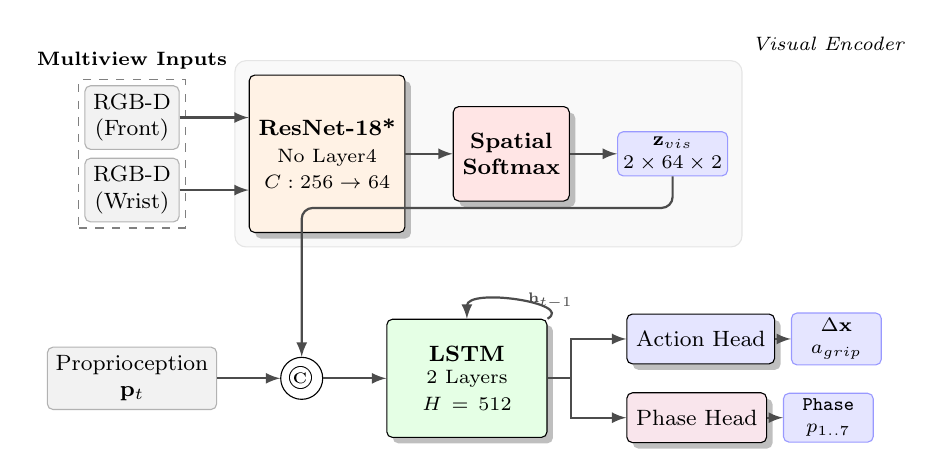
\begin{tikzpicture}[
    node distance=0.6cm and 0.6cm, % 减小节点间距
    font=\footnotesize, % 整体使用小号字体
    % 定义样式
    basic/.style={draw, rectangle, rounded corners=2pt, align=center},
    input/.style={basic, fill=gray!10, draw=gray!60, inner sep=3pt},
    module/.style={basic, fill=white, draw=black, drop shadow, minimum height=1.8em},
    tensor/.style={basic, fill=blue!10, draw=blue!40, inner sep=2pt, font=\scriptsize\ttfamily},
    operator/.style={circle, draw, fill=white, inner sep=1pt},
    arrow/.style={->, >=latex, thick, color=black!70}
]

    % ============================================================
    % Row 1: Visual Perception Pipeline (Left to Right)
    % ============================================================
    
    % 1. Inputs (Stacked)
    \node[input] (cam1) {RGB-D\\(Front)};
    \node[input, below=0.1cm of cam1] (cam2) {RGB-D\\(Wrist)};
    \node[fit=(cam1)(cam2), draw, dashed, color=gray, inner sep=2pt, label=above:\scriptsize \textbf{Multiview Inputs}] (input_group) {};

    % 2. ResNet
    \node[module, right=0.8cm of input_group, fill=orange!10, minimum height=2cm] (resnet) {\textbf{ResNet-18*}\\ \scriptsize No Layer4 \\ \scriptsize $C: 256 \to 64$};

    % 3. Spatial Softmax
    \node[module, right=0.6cm of resnet, fill=red!10, minimum height=1.2cm] (ssm) {\textbf{Spatial}\\\textbf{Softmax}};

    % 4. Visual Features (End of Row 1)
    \node[tensor, right=0.6cm of ssm] (z_vis) {$\mathbf{z}_{vis}$\\ \scriptsize $2 \times 64 \times 2$};

    % Arrows Row 1
    \draw[arrow] (cam1.east) -- (cam1.east -| resnet.west);
    \draw[arrow] (cam2.east) -- (cam2.east -| resnet.west);
    \draw[arrow] (resnet) -- (ssm);
    \draw[arrow] (ssm) -- (z_vis);

    % Background Box for Visual Encoder
    \begin{pgfonlayer}{background}
        \node[fit=(resnet)(ssm)(z_vis), fill=gray!5, rounded corners, draw=gray!20, inner sep=5pt, label=north east:\scriptsize \textit{Visual Encoder}] (enc_bg) {};
    \end{pgfonlayer}


    % ============================================================
    % Row 2: Sensor Fusion & Temporal Dynamics (Left to Right)
    % ============================================================
    
    % 1. Proprioception (Aligned below Inputs)
    \node[input, below=1.5cm of input_group] (prop) {Proprioception\\ $\mathbf{p}_t$};

    % 2. Concatenation Operator (Aligned below ResNet roughly)
    % Calculate position: horizontally between prop and where LSTM should be
    \node[operator, right=0.8cm of prop] (concat) {$\copyright$};

    % 3. LSTM (Aligned below Spatial Softmax roughly)
    \node[module, right=0.8cm of concat, fill=green!10, minimum height=1.5cm, text width=1.8cm] (lstm) {\textbf{LSTM}\\ \scriptsize 2 Layers\\ \scriptsize $H=512$};

    % 4. Heads (Aligned below z_vis)
    % Action Head
    \node[module, right=1.0cm of lstm, yshift=0.5cm, fill=blue!10] (head_action) {Action Head};
    \node[tensor, right=0.2cm of head_action, text width=1.0cm] (out_action) {$\Delta \mathbf{x}$\\$a_{grip}$};
    
    % Phase Head
    \node[module, right=1.0cm of lstm, yshift=-0.5cm, fill=purple!10] (head_phase) {Phase Head};
    \node[tensor, right=0.2cm of head_phase, text width=1.0cm] (out_phase) {Phase\\$p_{1..7}$};

    % ============================================================
    % Connections between Rows
    % ============================================================
    
    % Arrow from Visual Features (Row 1) down to Concat (Row 2)
    % We use a specific path to make it look clean
    \draw[arrow, rounded corners] (z_vis.south) -- ++(0,-0.4) -| (concat.north);
    
    % Proprioception to Concat
    \draw[arrow] (prop) -- (concat);

    % Concat to LSTM
    \draw[arrow] (concat) -- (lstm);
    
    % LSTM recurrent loop
    \draw[arrow] (lstm.north east) to[out=30,in=90] node[right, font=\tiny] {$\mathbf{h}_{t-1}$} (lstm.north);

    % LSTM to Heads
    \draw[arrow] (lstm.east) -- ++(0.3,0) |- (head_action.west);
    \draw[arrow] (lstm.east) -- ++(0.3,0) |- (head_phase.west);
    
    % Heads to Outputs
    \draw[arrow] (head_action) -- (out_action);
    \draw[arrow] (head_phase) -- (out_phase);

\end{tikzpicture}
\caption{\textbf{Architecture of the Vision-Final Policy.} To optimize for spatial constraints, the visual processing pipeline (top row) extracts geometric features ($\mathbf{z}_{vis}$), which are then fused with proprioception and processed by the temporal aggregation module (bottom row) to produce control actions and phase predictions.}
\label{fig:arch}
\end{figure*}

1.  {\bfseries Visual Encoder (ResNet-18 + Spatial Softmax):} 
    We modify a ResNet-18 backbone by adapting the first convolutional layer to accept 4-channel input (initializing the depth weight via mean-averaging RGB weights). We remove the final \textit{Layer4} to preserve spatial resolution and add a projection layer to reduce the channel dimension from 256 to $K=64$. \\ 
    To efficiently extract geometric features, we employ a {\bfseries Spatial Softmax} layer. For each feature map $k \in \{1...K\}$, it computes the expected 2D keypoint coordinates $(\mu_{x_k}, \mu_{y_k}) = \sum_{i,j} (i, j) \cdot \text{Softmax}(\mathbf{F}_k)_{ij}$. This compresses the visual representation into a compact feature vector $\mathbf{z}_{vis} \in \mathbb{R}^{2 \times K \times 2}$ (2 cameras $\times$ 64 points).

2.  {\bfseries Temporal Aggregation (LSTM):}
    The visual features are concatenated with the proprioception vector $\mathbf{p}_t$ and fed into a 2-layer LSTM with a hidden size of 512. The LSTM maintains a hidden state $\mathbf{h}_t$ to integrate history, effectively acting as a state estimator that filters sensor noise and tracks phase transitions.

3.  \textbf{Multitask Heads:} 
    The network outputs predictions via two parallel heads:
    \begin{itemize}
        \item \textbf{Action Head:} Predicts the end-effector delta position $\Delta \mathbf{x} \in \mathbb{R}^3$ and gripper action $a_{grip} \in [0,1]$.
        \item \textbf{Phase Head (Auxiliary):} Predicts the current sub-task phase $p_{phase} \in \{1...7\}$ (e.g., Approach, Grasp, Lift). This dense supervision forces the LSTM to explicitly model the logical structure of the task.
    \end{itemize}

\subsubsection{Loss Function}
The model is trained end-to-end using a composite objective function that balances trajectory tracking, grasp classification, and phase recognition:

\begin{equation}
\mathcal{L}_{total} = \lambda_{pos} \mathcal{L}_{Huber}(\Delta \mathbf{x}, \Delta \hat{\mathbf{x}}) + \lambda_{grip} \mathcal{L}_{BCE}(a, \hat{a}) + \lambda_{phase} \mathcal{L}_{CE}(p, \hat{p})
\end{equation}

where $\mathcal{L}_{Huber}$ is the Huber Loss (delta=1.0) for robust position regression, $\mathcal{L}_{BCE}$ is Binary Cross Entropy for gripper actuation, and $\mathcal{L}_{CE}$ is Cross Entropy for phase classification. Based on empirical tuning, we set the loss weights to $\lambda_{pos}=1.0$, $\lambda_{grip}=0.5$, and $\lambda_{phase}=0.2$. The model is optimized using the AdamW optimizer with a learning rate of $2 \times 10^{-4}$ and weight decay of $1 \times 10^{-3}$.

\subsection{Data Augmentaion}
To scale the limited set of real teleoperated trajectories into a large and diverse training corpus, we implemented a structured geometric augmentation pipeline inspired by MimicGen. The core idea is to decompose each demonstration into a chain of semantically meaningful subtasks, then recombine and perturb key elements while preserving task structure and physical feasibility. The augmentation process consists of the following steps:

{\bf Key-Frame Extraction}
For each subtask (e.g., approach, grasp, transport, align, release), we randomly sample representative key frames from the original trajectory. These key frames serve as anchor points for new trajectory compositions, ensuring that the augmented sequences still respect the high-level structural constraints of the task.

{\bf Interpolated Trajectory Construction}
Smooth interpolation (e.g., via cubic splines) connects the selected key frames. During interpolation, segment-wise Gaussian noise is applied with carefully tuned amplitudes. The perturbation schedule is designed to increase sample diversity while maintaining kinematic and dynamic plausibility, thereby encouraging the policy to learn robust behaviors rather than memorizing exact paths.

{\bf End-Effector Inverse Kinematics (IK) Re-solving}
After interpolation and perturbation, the resulting end-effector trajectory is re-solved using the robot’s IK solver. This step guarantees that all generated trajectories remain executable by the Franka Panda arm, discarding any kinematically invalid sequences.

{\bf Hand Action Replay}
Given the high dimensionality and tight constraints of multi-fingered or gripper actions, we adopt a direct replay strategy for finger/jaw commands. Hand actions are replayed exactly as in the original demonstration at corresponding key frames, without additional interpolation, to avoid introducing unrealistic distortions or grasp failures.

This procedure enables us to expand an initial set of 10 high-quality human teleoperated demonstrations into 1000 augmented trajectories, substantially broadening the distribution of states and actions seen during training.
\subsection{World model transfer}
\begin{figure}[ht]
\centering
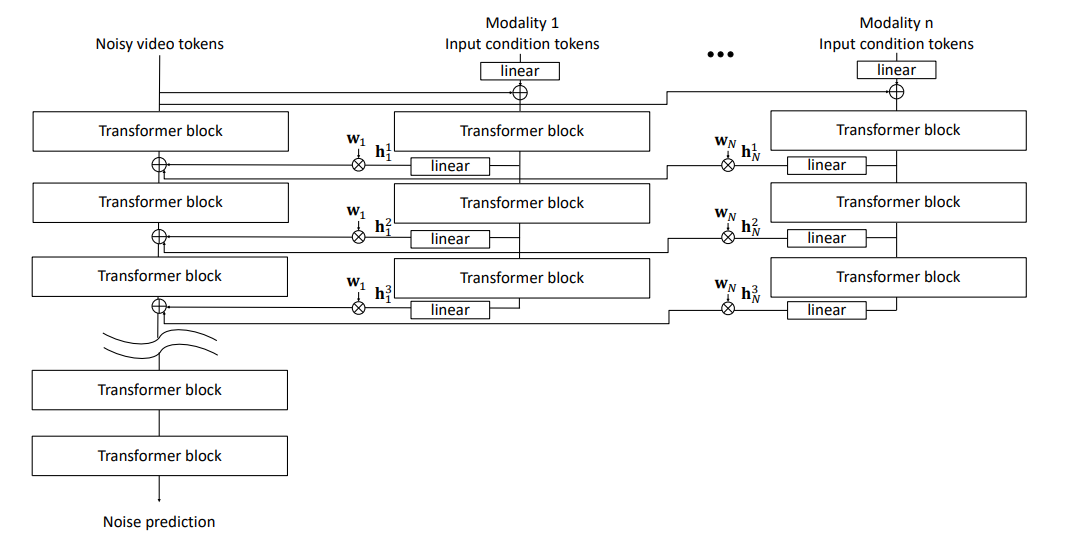
\includegraphics[width=0.95\columnwidth]{pic/cosmos transfer.png}
\caption{Cosmos-Transfer1 is a world generator with adaptive multimodal control. It contains multiple control
branches to extract control information from different modality inputs such as segmentation, depth, and edge.
}
\label{fig:cosmos transfer}
\end{figure}
To bridge the visual domain gap between simulation and reality, we employ Cosmos-Transfer, a powerful diffusion-based multimodal controllable world generator built by post-training the Cosmos-Predict foundation model.

Cosmos-Transfer takes multiple conditional input videos $(c_1, c_2, ..., c_n)$, each representing a different modality ( RGB, segmentation, depth, edge maps), and generates photorealistic simulated video sequences conditioned on these inputs\ref{fig:cosmos transfer}. For fine-grained spatiotemporal control, the model incorporates an adaptive spatiotemporal control map $w \in R^{H\times W\times T\times N}$, where $H$, $W$, and $T$ denote video height, width, and frame count, and $N$ is the number of modalities.

For each control branch $i$ and block $l$, intermediate activations $h_l^i$ are modulated by the corresponding slice of the control map $w_l^i$. The final contribution added back to the main diffusion branch is computed via element-wise multiplication:$w_l^i · h_l^i$.This adaptive fusion allows the model to dynamically emphasize the most informative modality in different spatial regions and time steps. 

In our pipeline, Cosmos-Transfer is used to stylize and diversify the visual appearance of augmented Isaac Sim trajectories (e.g., varying lighting, textures, backgrounds, and subtle rendering artifacts), producing photorealistic renderings that significantly reduce the perceptual sim-to-real gap for vision-based policies.
% \begin{center}
%    \url{http://www.iclr.cc/}
% \end{center}
% The file \verb+iclr2025_conference.pdf+ contains these
% instructions and illustrates the
% various formatting requirements your ICLR paper must satisfy.
% Submissions must be made using \LaTeX{} and the style files
% \verb+iclr2025_conference.sty+ and \verb+iclr2025_conference.bst+ (to be used with \LaTeX{}2e). The file
% \verb+iclr2025_conference.tex+ may be used as a ``shell'' for writing your paper. All you
% have to do is replace the author, title, abstract, and text of the paper with
% your own.

% The formatting instructions contained in these style files are summarized in
% sections \ref{gen_inst}, \ref{headings}, and \ref{others} below.

\section{Experiment}
\subsection{Evaluation of Training and Model Generalization}
\subsubsection{Architecture Comparison and Privileged Information Dependency}
We conducted large-scale comparative experiments in the PyBullet environment to rigorously assess training dynamics, model architectures, and generalization capabilities. To ensure statistical significance, the MLP-Base and final Vision-Final models were each evaluated over 500 independent runs with different random seeds, while all ablation baselines were tested over 200 runs.
Table 1 summarizes the key model configurations, input modalities, success rates, and qualitative analysis.Rather than binary success/failure evaluation, we designed a progressive “gradient of difficulty” test suite to probe the robustness boundaries of both privileged and visual policies.
\begin{table*}[t]
\centering
\caption{{\bfseries Architecture Comparison \& Performance.} We compare the privileged baseline against visual policies with varying input resolutions and configurations. $\mathcal{O}_{priv}$ denotes ground-truth physical states, while $\mathcal{O}_{vis}$ relies purely on pixels. Note that the low resolution ($64^2$) severely limits the spatial expressiveness of the CNN encoder.}
\label{tab:model_comparison}
\begin{tabular}{@{}llcccc@{}}
\toprule
{\bfseries Model} & {\bfseries Architecture} & {\bfseries Resolution} & {\bfseries Input Space} & {\bfseries Aux. Task} & {\bfseries Success Rate} \\ \midrule
\textsc{MLP-Base} & Residual MLP & N/A & $\mathcal{O}_{priv}$ & - & 98.6\% \scriptsize{(500 runs)} \\
\textsc{Vision-A} & CNN-LSTM & $64 \times 64$ & $\mathcal{O}_{vis} + \mathbf{x}_{obj}^{ee}$ & - & 100.0\% \\
\textsc{Vision-B} & CNN-LSTM & $64 \times 64$ & $\mathcal{O}_{vis}$ & - & 47.4\% \\
{\bfseries \textsc{Vision-Final}} & {\bfseries CNN-LSTM} & {\bfseries 112 $\times$ 112} & {\bfseries $\mathcal{O}_{vis}$} & {\bfseries Phase Pred.} & {\bfseries 84.8\%} \scriptsize{(500 runs)} \\ \bottomrule
\end{tabular}
\end{table*}

{\bfseries In-depth Analysis — Reactive Control vs. Temporal Reasoning:}  The 98.6\% success rate of MLP-Base reveals that the physical control problem is fundamentally simple when perfect privileged state information is available. The relative position vector $  (p_{\text{obj}} - p_{\text{ee}})  $ at each frame uniquely determines the next optimal action, rendering temporal memory unnecessary.
In contrast, visual observations (pixels) lack the Markov property due to occlusion, lighting variation, and perceptual ambiguity. Here, the LSTM serves not for long-horizon planning, but for state estimation and temporal smoothing: it integrates historical frames to denoise perception and implicitly models the task’s phase transition dynamics. Without LSTM, visual policies oscillate at critical boundaries (e.g., “almost grasped” vs. “grasped”), leading to frequent failures.

\textbf{Model Selection and Training Dynamics.} Prior to finalizing the architecture, we performed extensive ablation studies on regularization strategies, given the delicate balance between model capacity and generalization under the constrained 112×112 input resolution.

We compared three regularization regimes:

\begin{minipage}{\linewidth}
\begin{itemize}
\item No regularization → fastest convergence on training set, but catastrophic overfitting (success rate$ < 20\%$ on unseen initial configurations).
Mixed regularization (Dropout 0.2 + 2D-Dropout 0.2) → 78.4\% success rate. While noise-resistant, 2D-Dropout tends to erase entire feature blocks, causing loss of critical spatial semantics (e.g., object edges) and mild underfitting at low resolution.
\item Standard Dropout 0.3 → best balance at 84.8\% success rate. It effectively prevents over-reliance on specific textures while preserving intact spatial feature maps.
\end{itemize}
\end{minipage}

Due to the highly randomized physical environment (as described in Section 2.3), the model requires significantly longer training. Convergence remains oscillatory until ~100 epochs; stable peak performance is only reached after 200 epochs, allowing the network to fully digest the diverse data distribution.


\subsubsection{Ideal Privileged Instruction Policy (MLP-Base)}

This policy establishes a theoretical upper bound of 98.6\% using absolute privileged state information. To probe its limitations, we conducted an extensive gradient sweep across 12 distinct simulation parameters. {\bfseries The complete visualization of these success curves (Advanced Robustness Evaluation) is provided in Appendix~\ref{app:robustness}.}

\begin{figure*}[t]
\centering
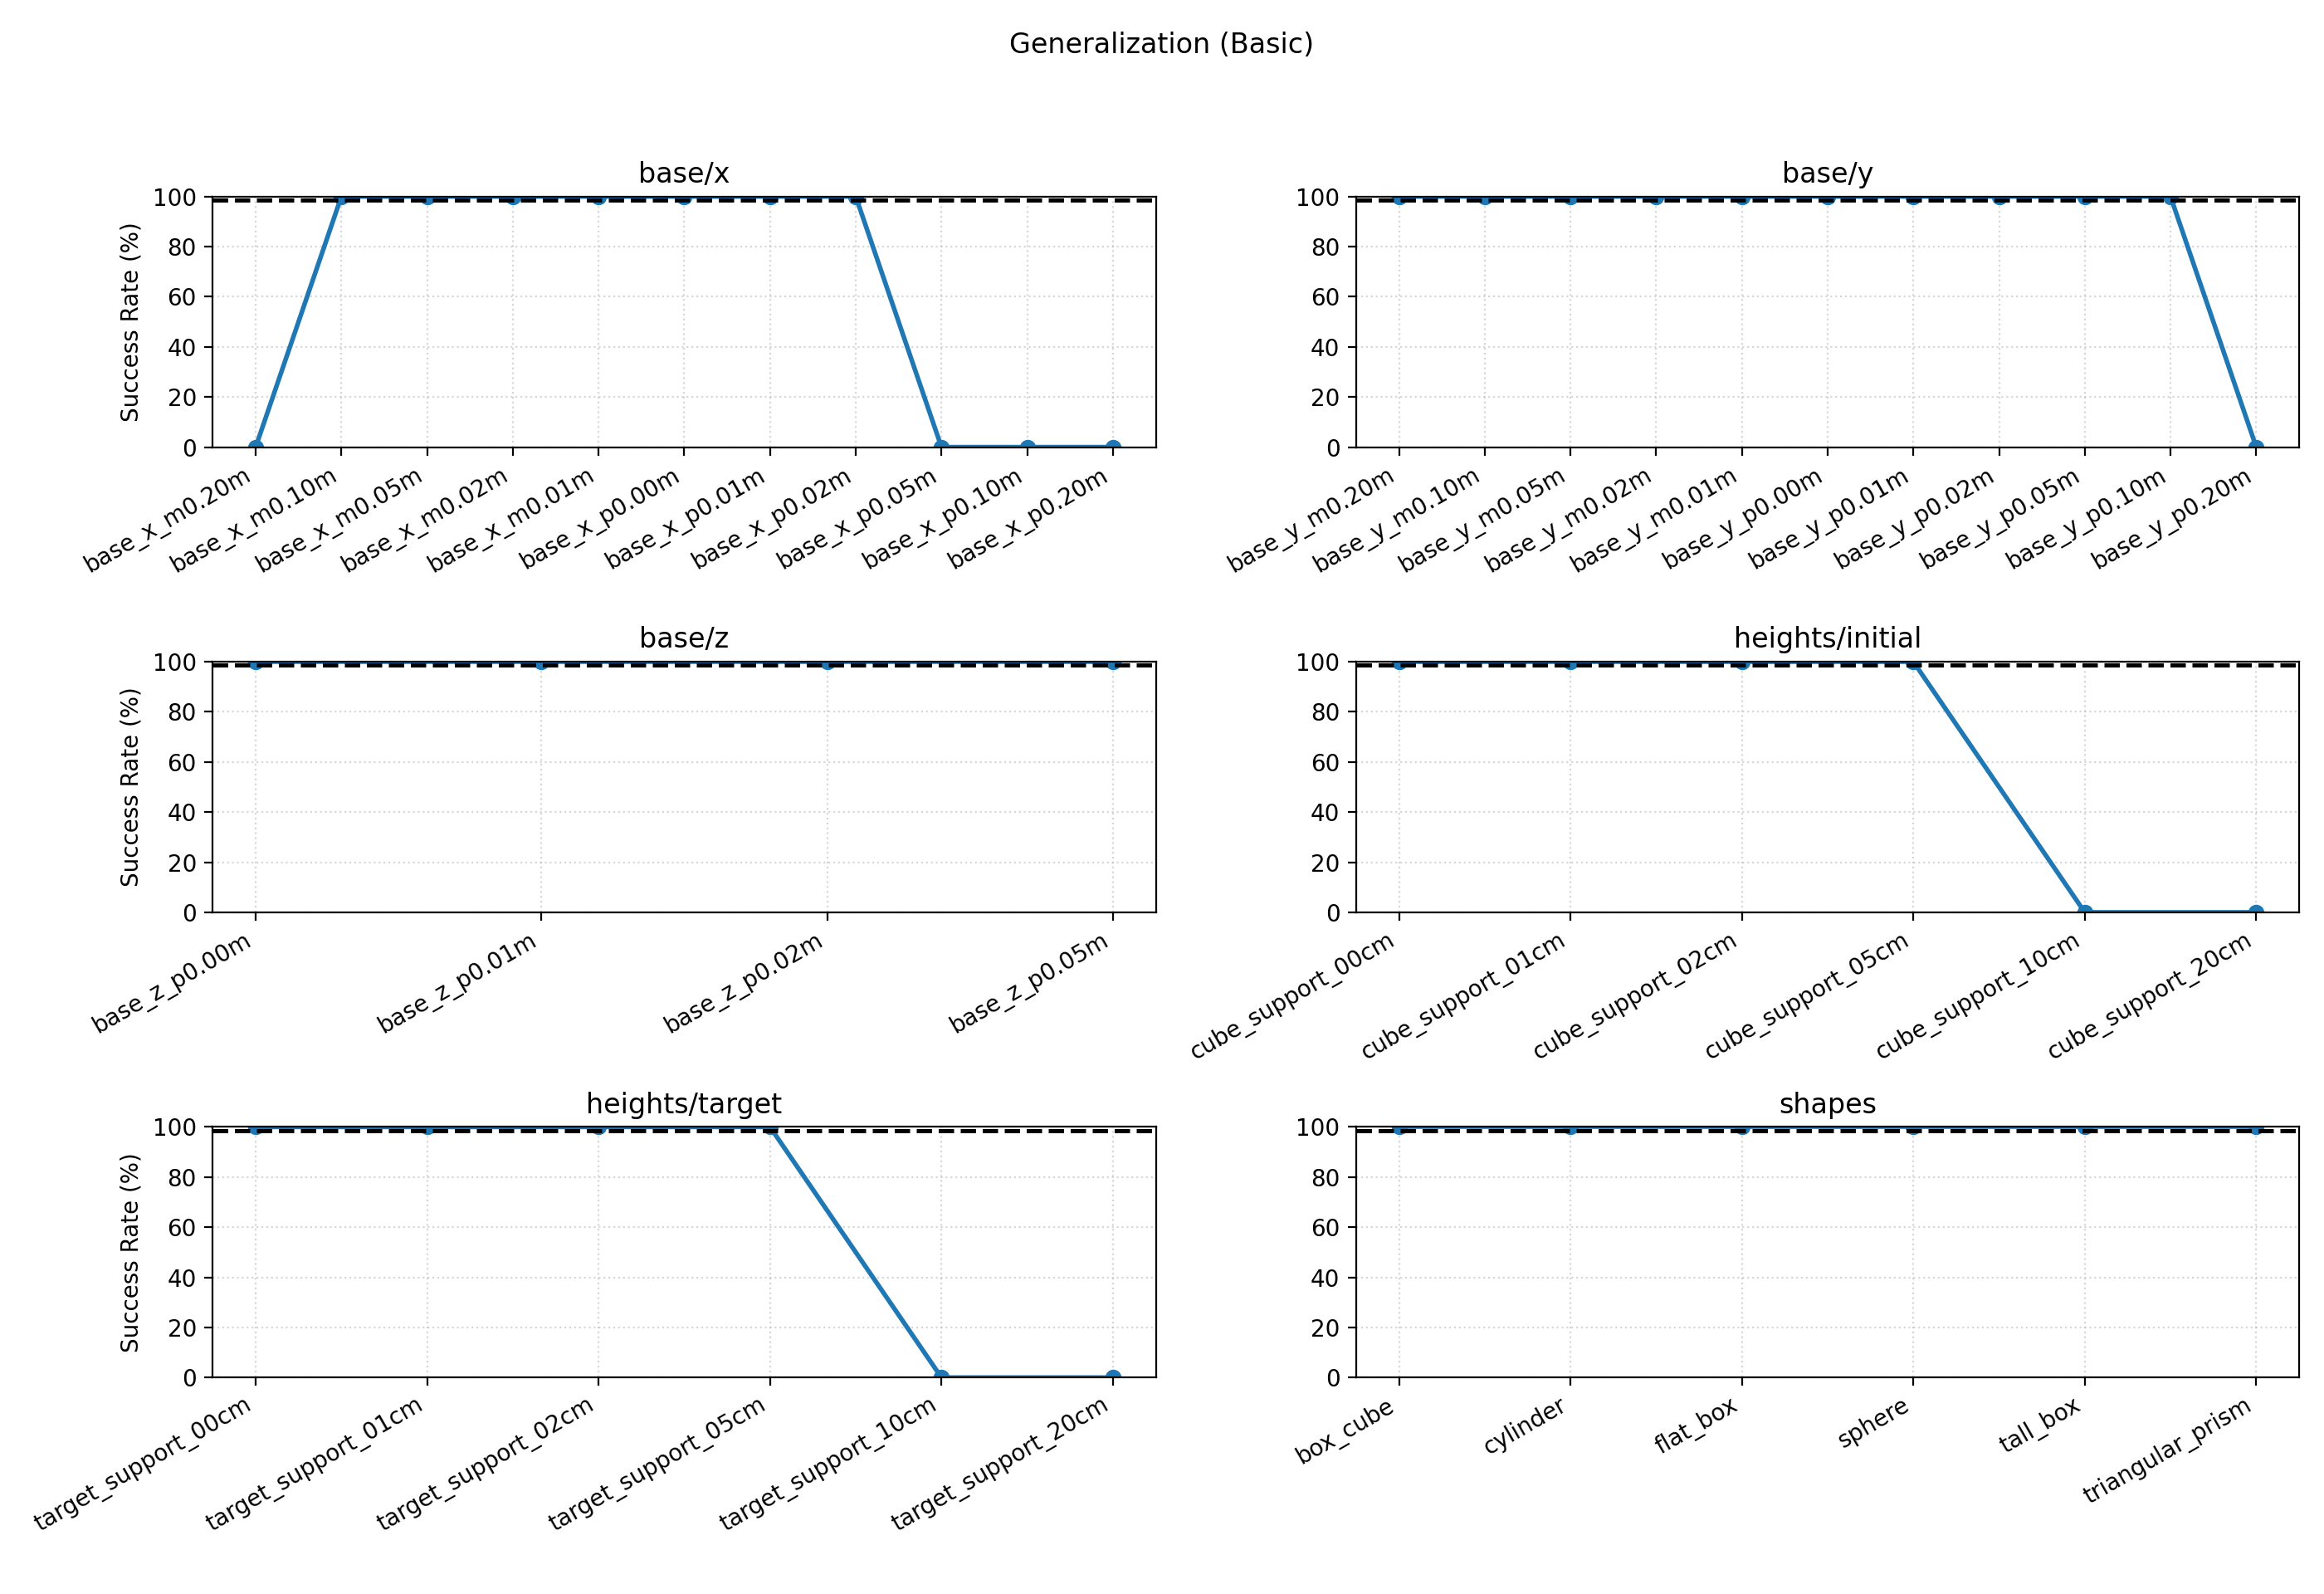
\includegraphics[width=\textwidth]{pic/Generalization(Basic).png}
\caption{{\bfseries Basic Generalization Evaluation (MLP-Base).} Success rates of the privileged policy across basic spatial variations including base position, initial/target heights, and object shapes. The policy shows strong geometric invariance but fails at hard spatial boundaries (e.g., height +10cm).}
\label{fig:gen_basic}
\end{figure*}

\textbf{Strengths: Perfect Invariance via State Abstraction.}
Geometric and appearance invariance: The policy achieves 100\% success across diverse object shapes (\texttt{box\_cube}, \texttt{cylinder}, \texttt{triangular\_prism}), as privileged observation abstracts objects to centroid coordinates, completely decoupling geometry, texture, and mesh complexity.
Physical parameter robustness: We observe no degradation under wide variations in friction ($0.5 \sim 5.0$), mass ($0.5\times \sim 1.5\times$), or external push disturbances (up to 5.0 N). The high-frequency (20 Hz) feedback loop enables strong compliance to dynamic changes.

\textbf{Weaknesses: Temporal \& Actuation Fragility.}
Despite its geometric robustness, the policy reveals critical vulnerabilities when simulation timing or actuation precision is altered. As summarized in \textbf{Table~\ref{tab:mlp_failure_modes}}, the stateless nature of the MLP leads to overfitting:

\begin{table}[h]
\centering
\small
\caption{{\bfseries Critical Failure Modes of MLP-Base.} While robust to physics, the policy collapses under temporal changes and execution noise (data extracted from Appendix).}
\label{tab:mlp_failure_modes}
\begin{tabular}{@{}lcc@{}}
\toprule
{\bfseries Parameter} & {\bfseries Condition} & {\bfseries Success Rate} \\ \midrule
{\bfseries Sim Timestep} & 240 Hz (Training) & 100\% \\
& 480 Hz (OOD) & {\bfseries 0\%} \\ \midrule
{\bfseries Action Noise} & $\sigma=0.000$ & 100\% \\
& $\sigma=0.010$ & {\bfseries 0\%} \\ \midrule
{\bfseries Height Offset} & +5 cm & 100\% \\
& +10 cm & {\bfseries 0\%} \\ \bottomrule
\end{tabular}
\end{table}

\begin{itemize}
    \item {\bfseries Severe overfitting to simulation timestep:} Perfect performance at 120 Hz and 240 Hz, but catastrophic failure (0\%) at 480 Hz. The learned action $\Delta pos$ is time-dependent rather than velocity-based; halving $\Delta t$ halves effective velocity, causing timeouts or dynamic failure.
    \item \textbf{Extreme sensitivity to action noise:} Success drops to 0\% with small action noise ($\sigma = 0.010$). As a stateless reactive controller, the MLP lacks the low-pass filtering capability of LSTM, making it unable to smooth high-frequency execution jitter.
\end{itemize}

{\bfseries Hard Spatial Generalization Boundary.}
The policy exhibits step-like failure: perfect at +5 cm height offset, but 0\% at +10 cm. This indicates memorization of training distribution mappings rather than true re-planning, leading to catastrophic forgetting outside the training support.

In summary, the privileged MLP demonstrates that reactive control can solve complex contact-rich dynamics perfectly when state is known, serving as an extremely strong teacher policy. However, its brittleness to timestep changes and actuation noise underscores the necessity of temporal memory or closed-loop smoothing for real-world deployment.


\subsubsection{Vision-Final Policy Generalization Analysis.}   
The final vision-based policy (ResNet-18 + LSTM, 112×112 RGBD input) achieves 84.8\% average success rate. We evaluated its robustness across five key dimensions.

\begin{figure*}[t]
\centering
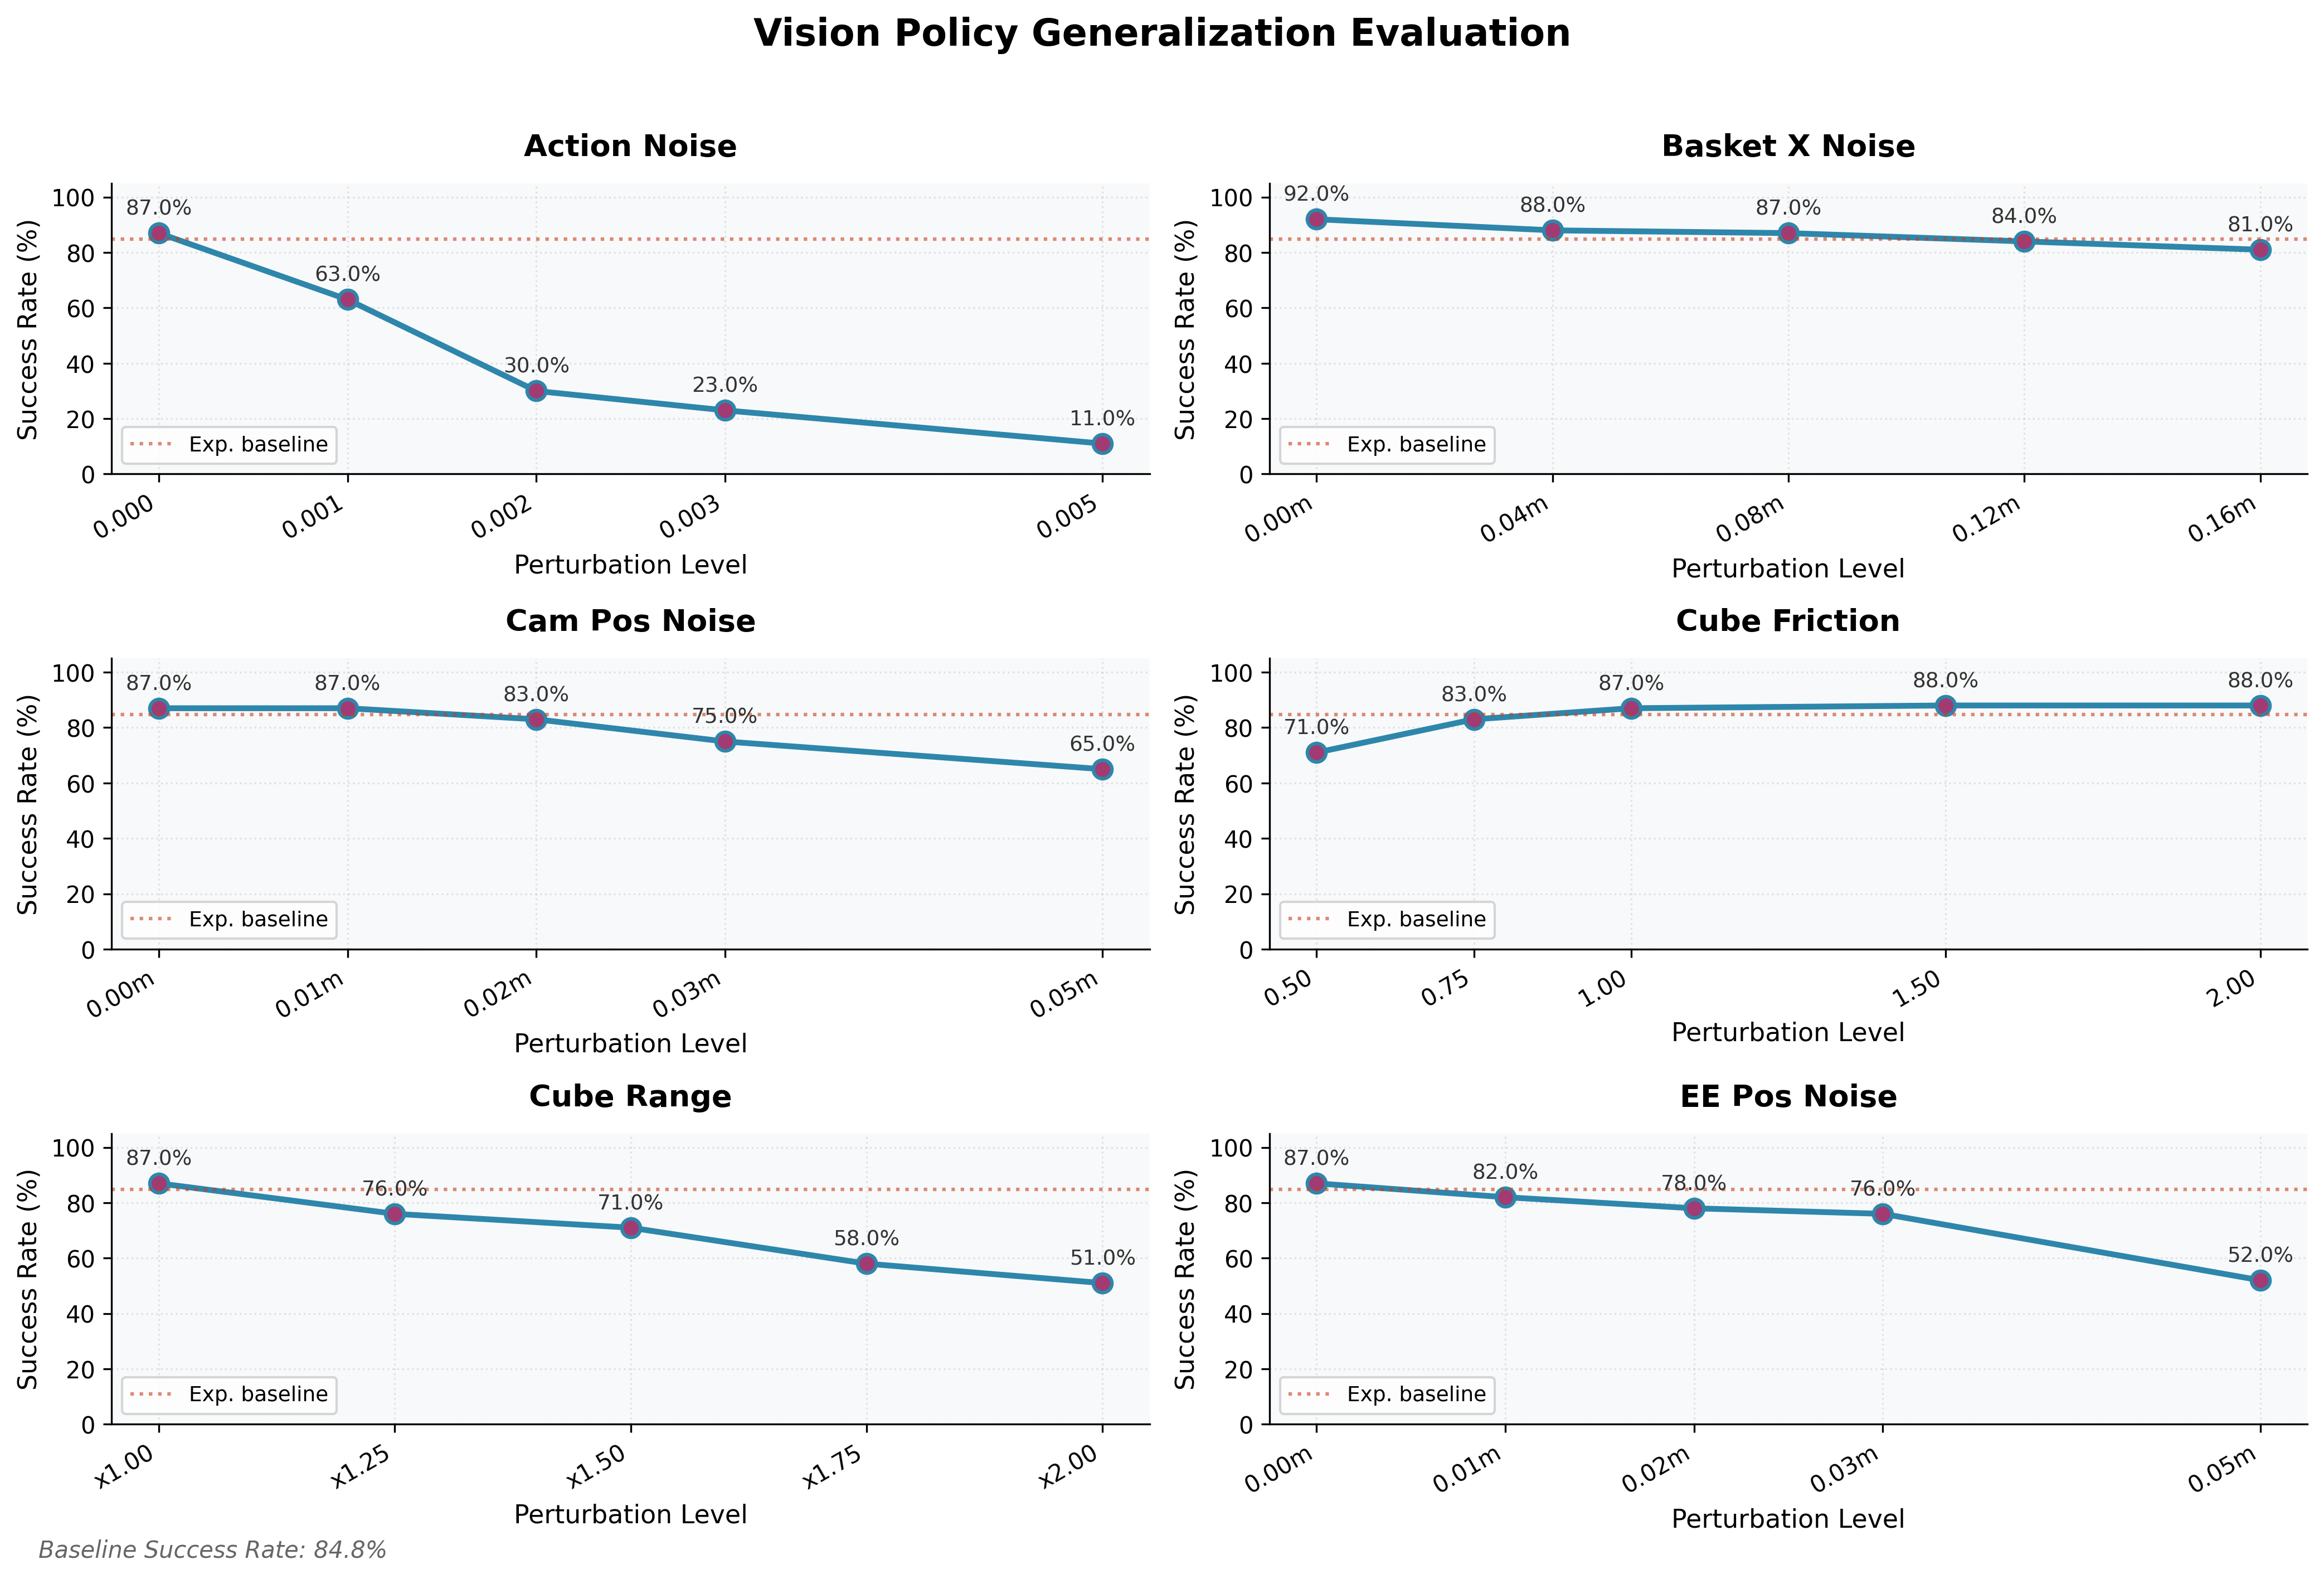
\includegraphics[width=\textwidth]{pic/Vision Policy Generalization Evaluation.png}
\caption{{\bfseries Vision Policy Generalization (Vision-Final).} Success rates under varying degrees of perturbation across six dimensions. The vision-based policy demonstrates strong robustness to visual noise (Camera Pose, Basket Position) and physical friction, but degrades linearly with spatial distribution shift (Cube Range) and shows high sensitivity to action execution noise.}
\label{fig:vision_eval}
\end{figure*}

{\bfseries Perceptual Robustness against Visual Perturbations.}    Camera pose noise (up to 5 cm displacement): success rate degrades gracefully from ~86\% to ~65\%, remaining nearly lossless within 2 cm. This indicates the model learns implicit visual servoing via Spatial Softmax rather than pixel memorization, showing promising sim-to-real potential.
Basket position noise (±16 cm): $>80\%$ success, directly attributable to the basket\_pos\_x\_noise randomization introduced during data collection.

{\bfseries Physical Adaptation.}   Friction sensitivity: Performance drops to ~70\% at low friction (0.5), due to delayed visual feedback and inability to perform microsecond-level contact adjustments. Stabilizes at ~88\% for friction $>1.0$, indicating effective action sequences when stable contact is feasible.

{\bfseries Spatial Distribution Shift.}    Cube initial area expansion (1.0× → 2.0× training range): near-linear success rate drop from 86\% to 50\%. Typical OOD failure: perspective distortion in extreme positions degrades ResNet spatial features, causing incorrect approach actions.

{\bfseries Action Execution Fragility.}    The most striking limitation is extreme sensitivity to action noise.The policy gets a ~30\% success rate with Gaussian noise std = 0.002,while dropping to ~10\%(near-total failure) with Gaussian noise std = 0.005.


Visual closed-loop introduces latency and uncertainty. Unlike the privileged MLP (which collapses only at std = 0.010), the vision policy requires much higher execution precision. Small high-frequency noise causes motion blur, feature jumps, and LSTM hidden-state divergence, resulting in oscillatory or misaligned behavior. This highlights a fundamental challenge of end-to-end visual control: achieving high-frequency stability under inherently noisy and ambiguous perception.

\subsubsection{Impact of Training Distribution on Generalization Capabilities}
\label{sec:dist_study}

To rigorously investigate the relationship between the \textit{generalization degree of the training dataset} and the \textit{generalization capability of the trained model}, we conducted a controlled study under a strictly constrained data budget. We defined a standardized ``Hard'' evaluation protocol (Baseline) characterized by maximum randomization parameters (Reset EE Noise = 40mm, Full Basket Noise, Full Cube Range). We then trained separate policies on datasets with varying degrees of distribution randomization (Scales/Levels) but limited to only 100 demonstrations each. The results, illustrated in Figure~\ref{fig:dist_study}, reveal three distinct generalization behaviors:

\begin{figure*}[t]
\centering
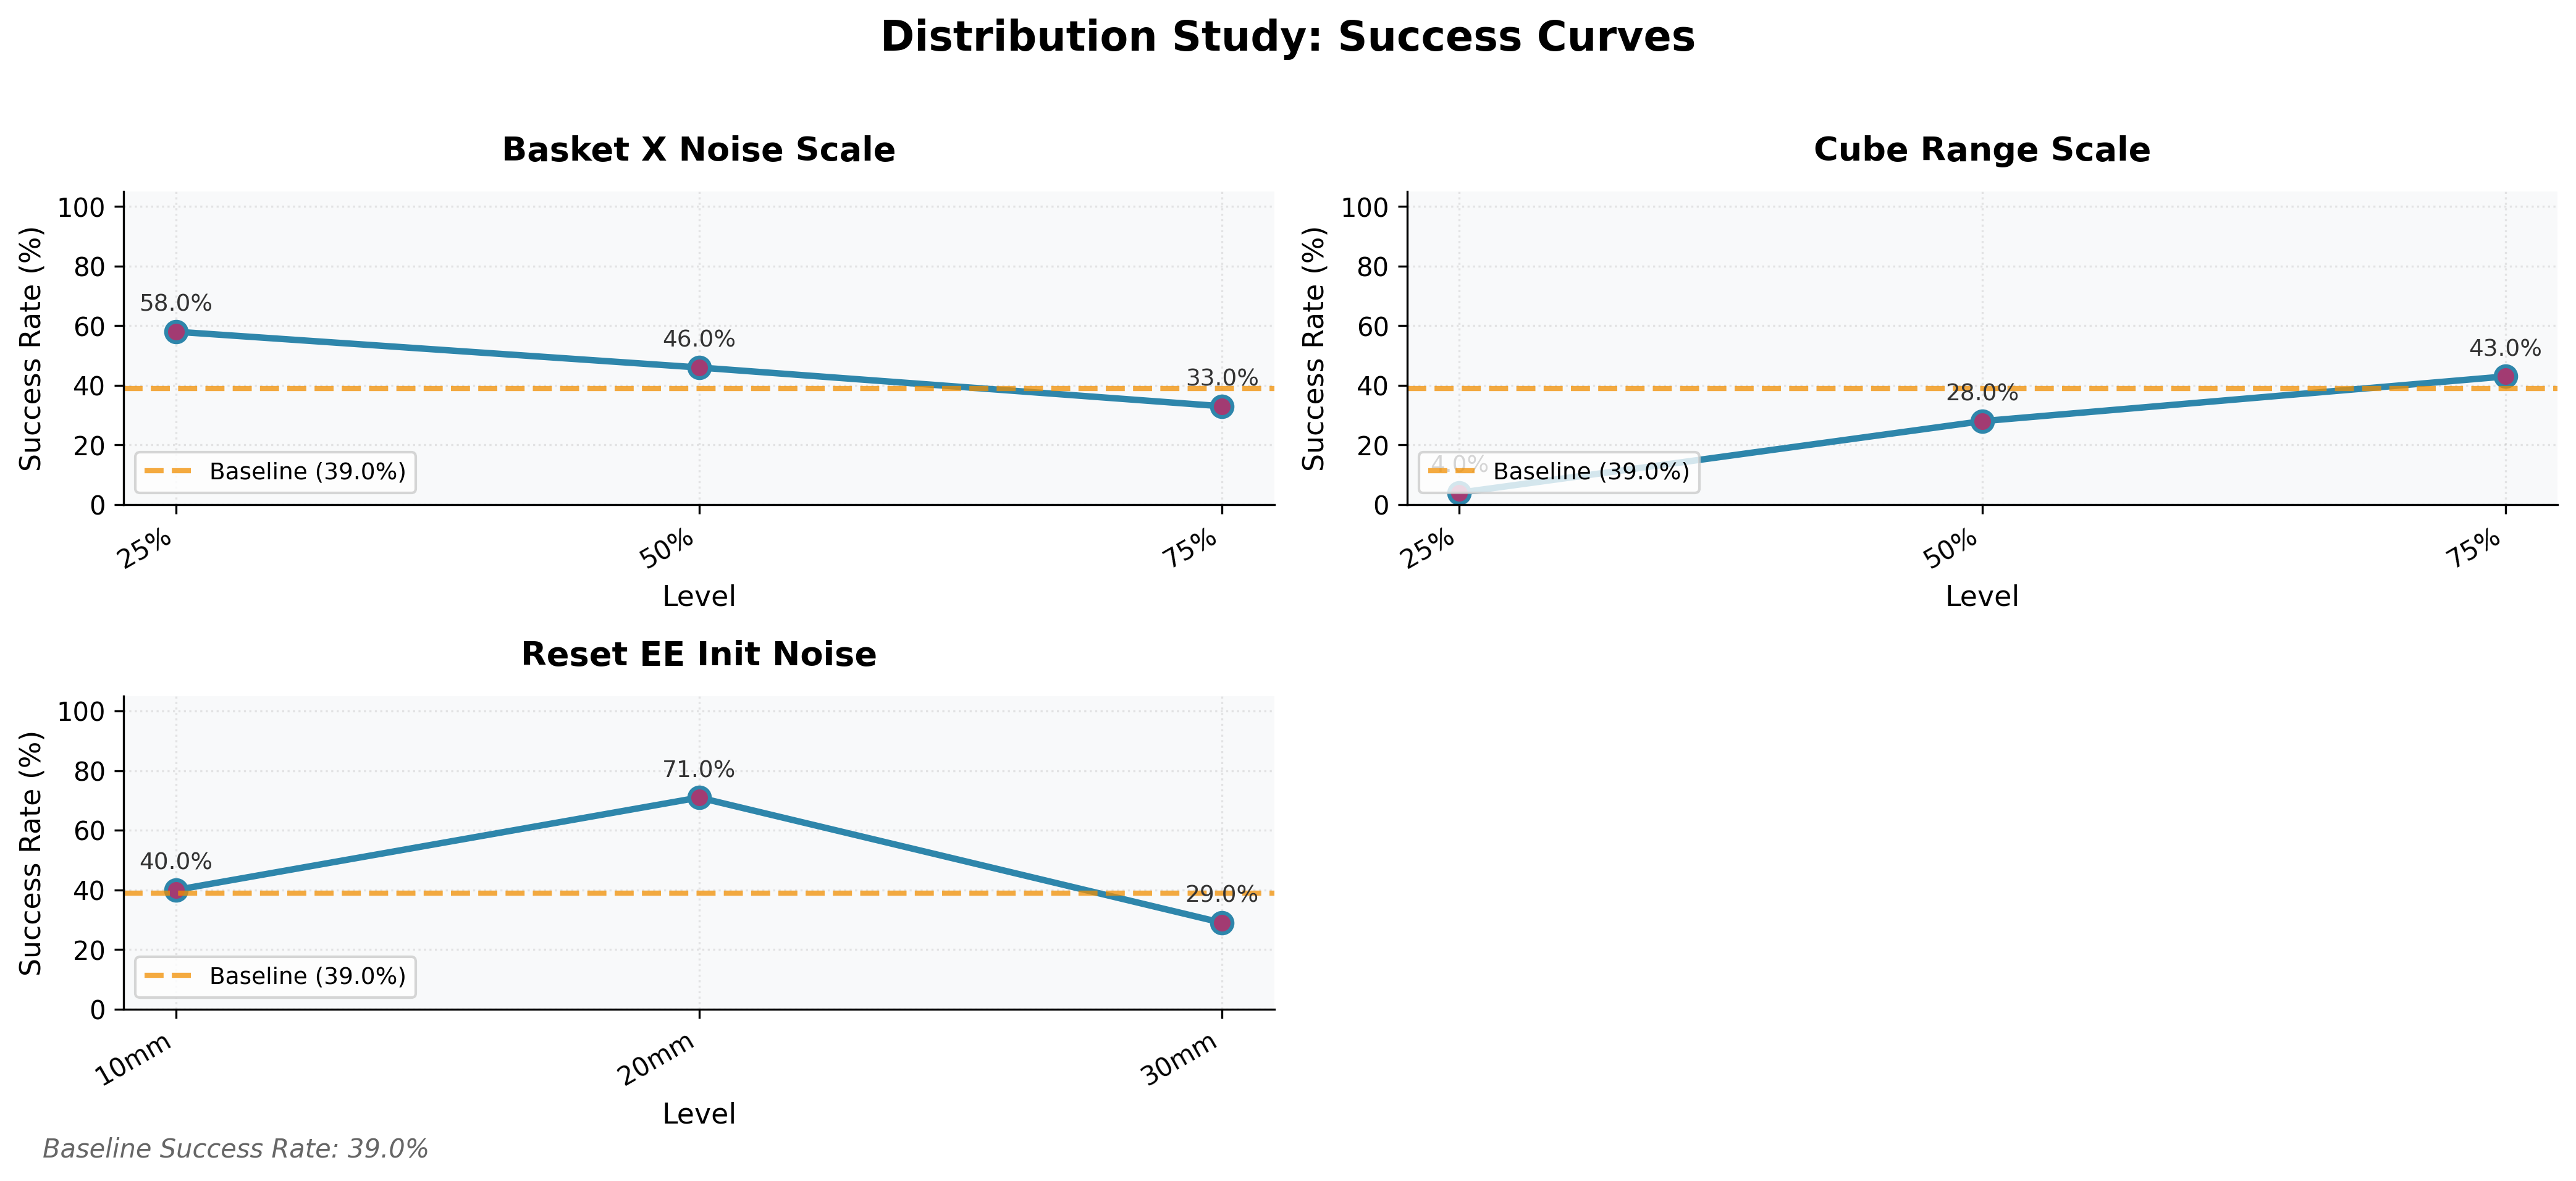
\includegraphics[width=\textwidth]{pic/Distribution_Study_Success_Curves.png}
\caption{{\bfseries Distribution Study: Training Distribution vs. Model Generalization.} Success rates on the fixed ``Hard'' baseline evaluation set when trained on datasets with varying randomization scales (limited to 100 demos). {\bfseries (Top Left)} Inverse scaling in basket noise suggests lower training variance aids feature learning under data scarcity. \textbf{(Top Right)} Direct scaling in spatial range confirms coverage is essential for geometric generalization. \textbf{(Bottom)} A ``sweet spot'' in initial condition noise (20mm) balances visual servoing learning against data sparsity.}
\label{fig:dist_study}
\end{figure*}

{\bfseries 1. Coverage-Dependent Generalization (Cube Range):}
As shown in the \textit{Cube Range Scale} plot, we observe a positive correlation between training distribution width and model performance. Training on a narrow distribution (25\%) results in near-zero success (4.0\%) on the hard evaluation set, confirming that for spatial positioning tasks, the model cannot extrapolate to out-of-distribution (OOD) regions. Expanding the training distribution is strictly necessary to encompass the test domain. However, collecting such large-scale, diverse real-world data is prohibitively expensive. This limitation motivates our transition to the Isaac Sim environment (Section 4.2), where we leverage MimicGen and Cosmos Transfer to synthetically scale up data diversity based on the insights gained from this section. 

{\bfseries 2. Stability-Inducing Generalization (Basket X Noise):}
Contraintuitively, the \textit{Basket X Noise Scale} plot demonstrates an inverse correlation. Training with reduced randomization (25\% level) yields a significantly higher success rate (58.0\%) on the fully randomized test set compared to training with full randomization (33.0\%). This suggests that under extreme data constraints (100 demos), high variance in target features prevents the model from converging on stable visual representations. A focused training distribution allows the model to learn robust heuristic features that generalize better than a model underfitted to a chaotic distribution.

{\bfseries 3. The "Sweet Spot" of Dynamic Correction (Reset EE Init Noise):}
The \textit{Reset EE Init Noise} curve exhibits a peak performance at the 20mm level (71.0\%). Training with minimal noise (10mm) leads to overfitting and open-loop behavior, failing to correct for large deviations in the test set. Conversely, excessive noise (30mm) disperses the limited data too thinly, hindering convergence. The 20mm setting represents an optimal balance, providing sufficient perturbation to induce closed-loop visual servoing behaviors without overwhelming the model's capacity.

These findings highlight that maximizing training randomization is not always optimal for generalization when data is scarce. Effective generalization requires balancing domain coverage with the learnability of the underlying signal.

% \label{gen_inst}

% The text must be confined within a rectangle 5.5~inches (33~picas) wide and
% 9~inches (54~picas) long. The left margin is 1.5~inch (9~picas).
% Use 10~point type with a vertical spacing of 11~points. Times New Roman is the
% preferred typeface throughout. Paragraphs are separated by 1/2~line space,
% with no indentation.

% Paper title is 17~point, in small caps and left-aligned.
% All pages should start at 1~inch (6~picas) from the top of the page.

% Authors' names are
% set in boldface, and each name is placed above its corresponding
% address. The lead author's name is to be listed first, and
% the co-authors' names are set to follow. Authors sharing the
% same address can be on the same line.

% Please pay special attention to the instructions in section \ref{others}
% regarding figures, tables, acknowledgments, and references.


% There will be a strict upper limit of 10 pages for the main text of the initial submission, with unlimited additional pages for citations. 
\subsection{Data enhancement pipeline}
\subsubsection{MimicGen-Based data augmentation}  
To address the data scarcity bottleneck for the more complex multi-step stacking task in Isaac Sim, we applied Isaac Lab,a geometry-aware trajectory augmentation framework — to scale up a small set of high-quality human teleoperated demonstrations.

We collected 10 source human demonstrations for the three-cube stacking task using Vision Pro teleoperation, as described in Section 2. Each demonstration was manually segmented into a chain of semantically meaningful subtasks. Following the general heuristic that tasks should be decomposed into the minimal number of subtasks necessary to still faithfully represent the full behavior, we divided the stacking sequence into three core subtasks.
This minimal decomposition balances task coverage and trajectory smoothness: too many subtasks increase the number of splicing points, which can introduce motion discontinuities and elevate the failure rate of generated demonstrations; too few subtasks reduce augmentation diversity.

MimicGen employs linear interpolation to bridge and concatenate subtask segments from different source demonstrations. The number of interpolation steps between key frames is a tunable hyperparameter that controls the smoothness of the resulting trajectories. For tasks with large object reset distributions (as in our stacking scenario), larger inter-segment gaps require more interpolation steps to produce kinematically smooth and dynamically plausible motions. Conversely, smaller gaps benefit from fewer steps to avoid unnecessary delays or over-smoothing.

Using an NVIDIA RTX 4090 GPU, we generated 1000 augmented trajectories from the original 10 demonstrations in approximately 1 hour. The overall success rate of the generated interpolation trajectories (i.e., trajectories that remained kinematically valid and collision-free after IK re-solving) was 72.3\%. Invalid trajectories were filtered out before training.

To investigate the scaling effect of augmented data volume on imitation learning performance, we further generated 2000 augmented trajectories from the same 10 source demonstrations using the same pipeline and trained separate policies on both datasets.

Evaluation was conducted under the same fully randomized initial pose conditions used for the baseline (randomization applied to all three cubes within a 0.2 × 0.2 m area). The results are summarized in Table~\ref{tab:mimicgen_scaling}.

\begin{table}[ht]
\centering
\caption{Impact of MimicGen data augmentation scale on stacking task success rate.}

\begin{tabular}{l c c}
\toprule
{\bfseries Training Dataset} & {\bfseries Number of Trajectories} & {\bfseries Success Rate (\%)} \\
\midrule
MimicGen 1k & 1000  & 60.0 \\
MimicGen 2k & 2000  & {\bfseries 97.0} \\
\bottomrule
\label{tab:mimicgen_scaling}
\end{tabular}
\end{table}

The substantial jump from 62.0\% to 96.6\% success rate when doubling the augmented dataset size clearly demonstrates the strong positive scaling effect of data volume in imitation learning, even when the additional trajectories are synthetically generated via geometric interpolation. This result underscores that, for contact-rich, multi-step manipulation tasks such as stacking, increasing demonstration diversity and quantity through automated augmentation is highly effective at improving policy robustness and reducing sensitivity to the narrow initial data distribution.

These findings complement our earlier PyBullet experiments, where distribution augmentation via object randomization and noise injection yielded similar generalization gains, and reinforce the central role of scalable, high-quality synthetic data generation in overcoming the fundamental data bottleneck of imitation learning for real-world robotic manipulation.
\subsubsection{Cosmos data augmentation}  
To further reduce the perceptual sim-to-real gap and enhance the robustness of vision-based policies to real-world variations in lighting, textures, backgrounds, and rendering styles, we explored the use of Cosmos-Transfer 1.0 (7B parameter model), the official controllable world generator released by NVIDIA in 2025.

In our pipeline, we first converted the geometrically augmented trajectories (generated via MimicGen from the 10 human teleoperated stacking demonstrations) into short MP4 video clips rendered from the robot’s wrist-mounted RGB-D camera perspective in Isaac Sim. These synthetic clips served as the base input videos. We then applied Cosmos-Transfer to perform background and appearance stylization, using the following multimodal conditioning inputs:

\begin{minipage}{\linewidth}
\begin{itemize}
\item Original RGB video (source appearance)
\item Semantic segmentation masks (object and scene layout)
\item Depth maps (3D structure)
\end{itemize}
\end{minipage}

The goal was to generate visually diverse variants of each trajectory — for example, changing indoor lighting conditions (daylight, warm/cool artificial light), background scenes (office, warehouse, kitchen), surface textures (wood, metal, plastic), and subtle rendering differences,while keeping the robot motion, object positions, and task progression intact.

Unfortunately, the inference process proved computationally intensive. Generating a single stylized video clip (typically 10–20 seconds long at 30 fps) required approximately 20 minutes of inference time on an NVIDIA RTX 4090 GPU, even with the 7B model. Given the limited project timeline and computational resources, we were unable to produce a large-scale augmented dataset (e.g., hundreds or thousands of stylized trajectories) sufficient for full end-to-end policy training and quantitative evaluation of generalization gains.

As a result, we could not yet empirically verify the downstream training effectiveness of Cosmos-Transfer–generated data on policy robustness in the stacking task. Nevertheless, we demonstrate the qualitative capability of the model through representative examples.
\begin{figure*}[t]
\centering
\begin{subfigure}[b]{0.24\textwidth}
    \centering
    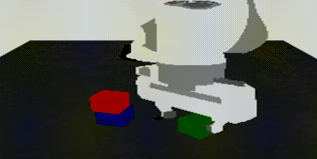
\includegraphics[width=\textwidth]{pic/rgb.png}
    \caption{RGB}
    \label{fig:rgb}
\end{subfigure}
\hfill
\begin{subfigure}[b]{0.24\textwidth}
    \centering
    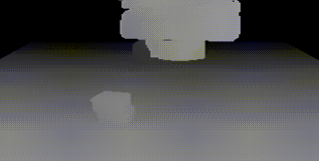
\includegraphics[width=\textwidth]{pic/depth.png}
    \caption{Depth}
    \label{fig:depth}
\end{subfigure}
\hfill
\begin{subfigure}[b]{0.24\textwidth}
    \centering
    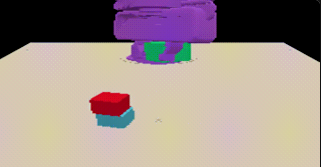
\includegraphics[width=\textwidth]{pic/seg.png}
    \caption{Segmentation}
    \label{fig:seg}
\end{subfigure}
\hfill
\begin{subfigure}[b]{0.24\textwidth}
    \centering
    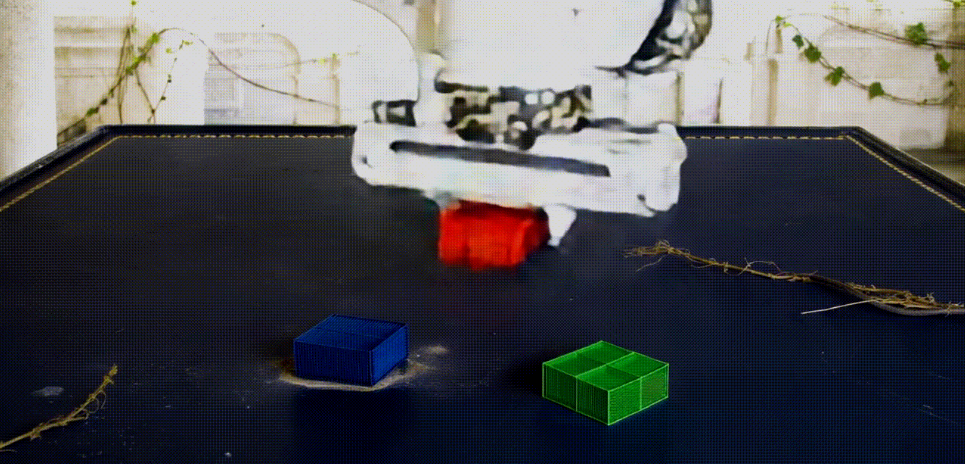
\includegraphics[width=\textwidth]{pic/output.png}
    \caption{Output}
    \label{fig:output}
\end{subfigure}
\caption{Qualitative results of Cosmos-Transfer 1.0. {\bfseries Top row}: Multimodal conditioning inputs (RGB, Depth, and Semantic Segmentation) from one representative frame of the original Isaac Sim trajectory. {\bfseries Bottom row}: Stylized output frames generated by Cosmos-Transfer, demonstrating diverse photorealistic appearance transfer while preserving robot motion and scene geometry.}
\label{fig:cosmos_transfer_qualitative}
\end{figure*}
\section{Results \& Discussion}

Our experiments reveal a clear dichotomy in the performance of imitation learning policies for robotic manipulation: privileged-state policies achieve near-perfect results in controlled settings, while vision-based policies demonstrate substantial robustness gains through targeted generalization techniques, yet remain vulnerable to specific forms of distribution shift and execution noise.

The privileged  MLP-Base  policy establishes an upper bound of  98.6\%  success under ideal conditions, excelling in scenarios with precise, noise-free state information. It exhibits perfect invariance to geometric variations (shape, texture, appearance), wide ranges of physical parameters (friction 0.5–5.0, mass scaling ±50\%, external pushes up to 5 N), and moderate spatial perturbations within the training distribution. This confirms that, when provided with oracle-level privileged information, the task is fundamentally simple from a control perspective: reactive, memory-free mapping suffices to solve complex contact-rich dynamics with high-frequency feedback.

In stark contrast, the vision-based  Vision-Final  policy (ResNet-18 + LSTM), trained without any privileged information, achieves a robust  84.8%  success rate in fully randomized environments — a remarkable result given the high-dimensional, noisy nature of RGB-D inputs. It performs particularly well in the following scenarios:

\begin{minipage}{\linewidth}
\begin{itemize}
\item Moderate perceptual disturbances: camera pose jitter up to ~2 cm causes almost no degradation, and up to 5 cm still yields ~65% success, thanks to implicit visual servoing enabled by Spatial Softmax.  
\item Target localization under randomization: $>80\%$ success with basket displacement of ±16 cm, directly attributable to training-time randomization of basket position.  
\item Reasonable physical conditions: stable performance $(~88\%)$ when friction coefficients exceed 1.0, indicating effective action sequences when stable contact can be established.
\end{itemize}
\end{minipage}

These strengths highlight the perceptual resilience of end-to-end visual policies, which can adapt to real-world-like variations in viewpoint and scene layout — capabilities entirely absent in pure coordinate-based MLP policies.

However, the vision policy exhibits sharp performance degradation in several critical regimes:

\begin{minipage}{\linewidth}
\begin{itemize}
\item Extreme spatial extrapolation (OOD): success rate drops linearly to $~50\%$ when initial object placement area doubles beyond the training distribution, due to severe perspective distortion and feature degradation at distribution edges.  
\item Low-friction regimes: drops to $~70\%$ at $\mu = 0.5$, as visual feedback latency prevents microsecond-scale corrections that privileged policies achieve effortlessly via contact sensing.  
\item Action execution noise: catastrophic failure even at very low levels (std = 0.002 → $30\%$; std = 0.005 → $~10\%$), an order of magnitude more sensitive than the privileged baseline. High-frequency jitter causes motion blur, feature jumps, and LSTM state divergence, trapping the arm in oscillatory or misaligned behaviors.
\end{itemize}
\end{minipage}

These failure modes underscore the fundamental limitations of pure imitation learning: extreme sensitivity to distribution shift, inability to recover from perturbations not present in demonstrations, and compounding errors due to the lack of an explicit reward signal that could guide recovery or exploration.

The proposed techniques proved highly effective in mitigating many of these limitations. High-resolution inputs ($112 \times 112$), Spatial Softmax for precise spatial feature extraction, dense 9-phase supervision, and standard Dropout 0.3 together lifted vision performance from a collapsed  47.4\%  (low-res baseline) to  84.8\%  under full randomization. Training-time object and target randomization successfully forced the policy to rely on visual anchoring rather than memorization.

For the more complex stacking task, MimicGen geometric augmentation demonstrated strong scaling behavior: increasing augmented trajectories from 1000 to 2000 raised success from  62.0\%  to  96.6\% , confirming that even synthetically interpolated data substantially improves robustness for multi-step, contact-rich tasks.

While computational constraints prevented large-scale quantitative evaluation of Cosmos-Transfer–generated visual variants, qualitative results show excellent preservation of kinematics with realistic transfer of lighting, textures, and backgrounds, suggesting that world-model-based visual augmentation holds great promise for closing the perceptual sim-to-real gap when inference efficiency improves.

Imitation learning offers clear advantages in simulation: it is simple to implement, data-efficient when demonstrations are available, and capable of achieving high performance with minimal engineering compared to reward-shaped RL. However, its brittleness to distribution shifts, lack of recovery mechanisms, and over-reliance on demonstration coverage severely limit real-world deployment. The measures we employed — randomization, dense supervision, geometric augmentation, and (prospectively) visual domain stylization — are effective steps toward more robust vision policies, yet the core challenges of OOD generalization and execution robustness remain open. Future progress likely lies in hybrid approaches that combine imitation pre-training with limited online RL fine-tuning, larger-scale synthetic data generation, and world-model-assisted recovery mechanisms. These small-scale experiments, even on seemingly simple tasks, starkly expose the profound difficulties that embodied intelligence still faces when moving from controlled simulation to the unstructured physical world.
\section{Conclusion \& Future Work}
This work systematically explores and evaluates several critical factors that influence the training effectiveness and generalization capability of imitation learning for robotic manipulation, including model architecture choices, data distribution diversity, regularization strategies, and data volume scaling. Through a carefully designed set of experiments on both simple pick-and-place and more complex multi-step stacking tasks, the study serves as a comprehensive case study that reveals core challenges in applying imitation learning to embodied robotic systems.

Thus, to the central question posed by the project — “How difficult is it to train a robotic arm to perform a simple task via imitation learning in a controlled simulation?” — the answer is clear: it may seem easy to train, often achieving near-perfect performance when privileged information or perfectly aligned demonstrations are available. However, improving generalization remains a fundamental challenge. Even modest distribution shifts — whether in spatial layouts, physical parameters, perceptual conditions, or execution noise — can cause sharp performance degradation, particularly for vision-based policies that must operate without oracle-level state information. These observations highlight that the apparent simplicity of imitation learning in idealized simulation environments masks profound difficulties when policies are expected to transfer to more diverse, noisy, or real-world-like conditions.

The proposed generalization-enhancing measures — high-resolution visual representations, spatial feature extraction, dense phase supervision, training-time randomization, and scalable geometric data augmentation — proved effective in pushing vision policies toward more robust performance. Nonetheless, persistent vulnerabilities to out-of-distribution spatial extrapolation, low-friction regimes, and especially high-frequency action noise underscore that imitation learning alone, without additional mechanisms for recovery or exploration, is insufficient for reliable real-world deployment.

Looking ahead, several promising directions can further advance imitation learning for robust robotic manipulation:

\begin{minipage}{\linewidth}
\begin{itemize}
\item Model architecture optimization: Diffusion Transformers (DiT) and related generative architectures show strong potential to better handle diverse, multimodal demonstration data and exhibit superior out-of-distribution generalization compared to traditional CNN-LSTM pipelines. While training such models remains computationally demanding, their ability to model complex distributions natively makes them a compelling candidate for future scaling.
\item Data distribution enhancement: Continued investment in domain randomization during data collection, combined with world-model-based background and appearance stylization (e.g., leveraging controllable generative models like Cosmos-Transfer), can produce more photorealistic and perceptually diverse training corpora, significantly narrowing the visual sim-to-real gap.
\item Data volume scaling: Automated trajectory augmentation via geometric interpolation (as demonstrated with MimicGen) and future integration of world-model-generated full trajectories offer scalable paths to orders-of-magnitude larger datasets, which empirical scaling laws suggest will yield substantial robustness improvements even for complex multi-step tasks.
\end{itemize}
\end{minipage}

By addressing these directions, future research can progressively close the gap between simulation-trained imitation policies and deployable, general-purpose robotic manipulation systems. Ultimately, this small-scale study on seemingly simple tasks serves as a microcosm of the broader embodied intelligence challenge: achieving reliable, adaptive behavior in the physical world remains one of the most profound open problems in robotics and AI.

\bibliography{iclr2025_conference}
\bibliographystyle{iclr2025_conference}


\appendix
\section{Appendix}

\subsection{Detailed Robustness Evaluation}
\label{app:robustness}

In this section, we provide the comprehensive visualization of the "Advanced Robustness Evaluation" for the MLP-Base policy, as discussed in Section 4.1.2. 

Figure~\ref{fig:gen_extra_full} illustrates the success rate curves across 12 different perturbation dimensions. While the policy demonstrates strong invariance to physical parameters (friction, mass, scale), it exhibits catastrophic failures under temporal shifts (simulation timestep) and actuation noise, confirming the limitations of stateless reactive control.

\begin{figure*}[htbp]
    \centering
    % 这里的 height 可以设大一点，让图更清楚
    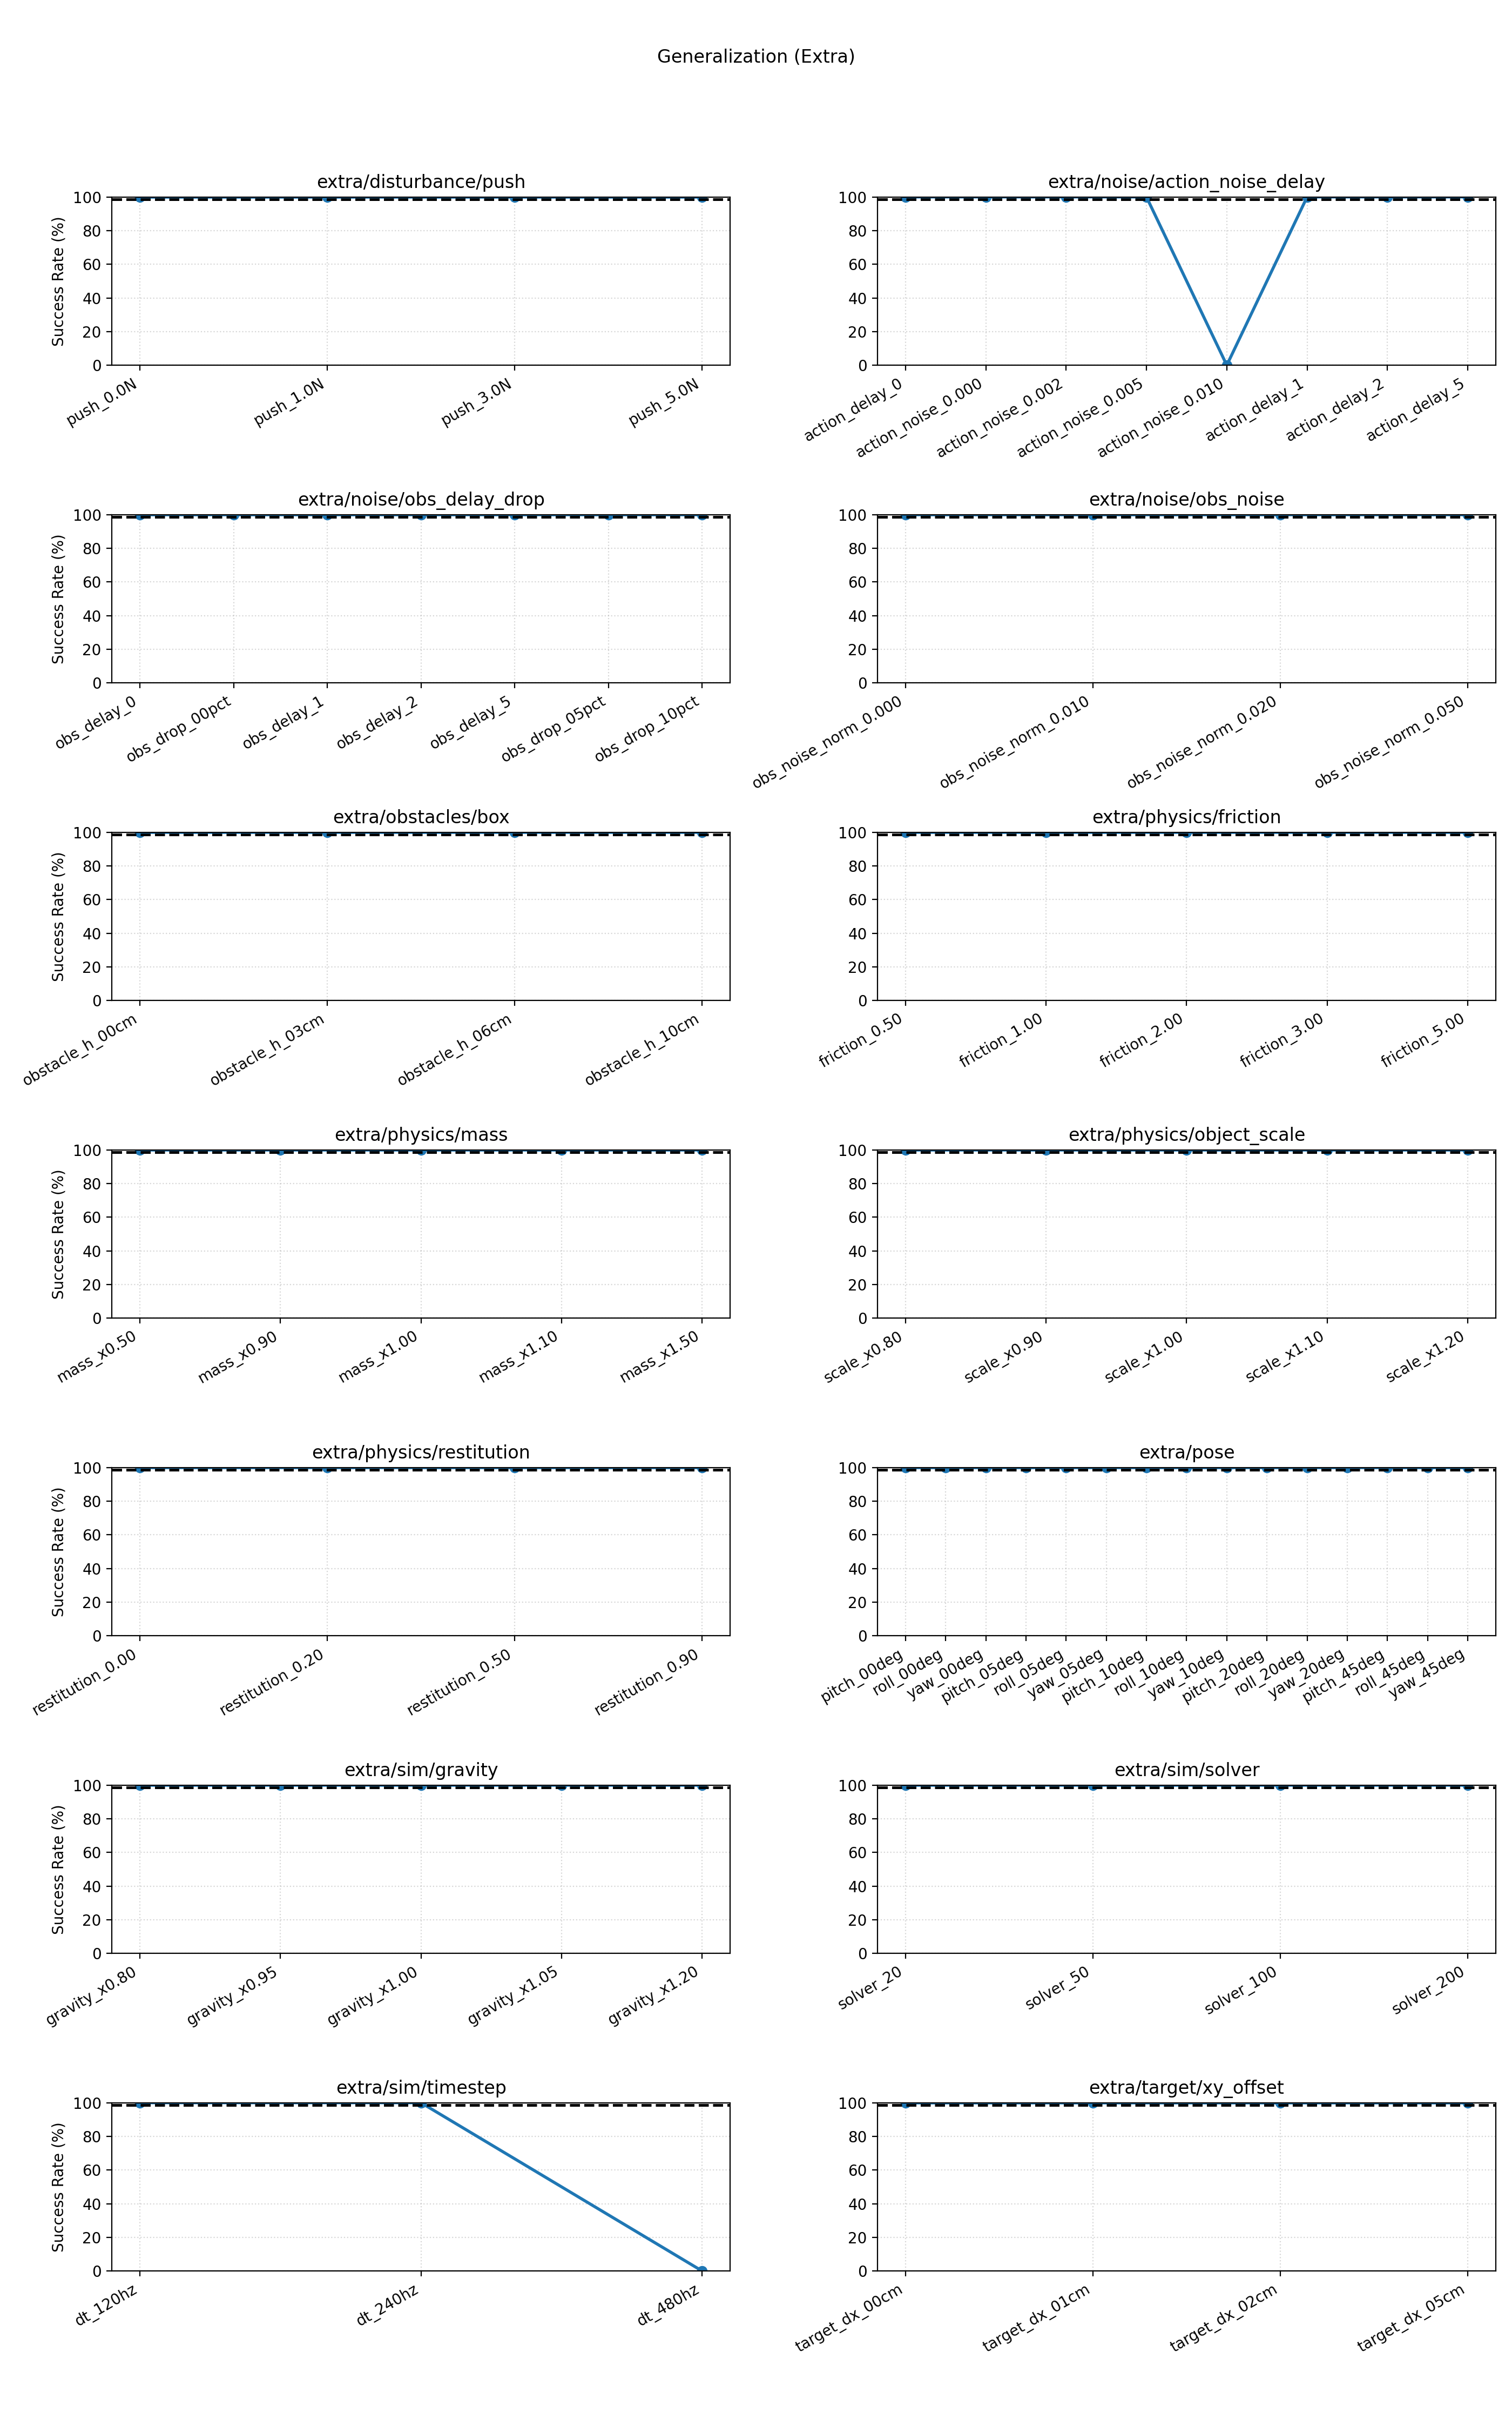
\includegraphics[width=0.78\textwidth]{pic/Generalization(Extra).png}
    \caption{{\bfseries Full Sweep of Robustness Tests (MLP-Base).} Detailed success rate curves across varying disturbances, physics parameters, and sensor/actuation noise levels. Note the sharp drop-off in the \texttt{timestep} and \texttt{action\_noise} subplots.}
    \label{fig:gen_extra_full}
\end{figure*}
% ==================== 附录结束 ====================

\end{document}


